\part{Weighted digraphs and optimization problems}
\label{ch:weighted}

\chapter{Weighted graphs, the single-source shortest paths problem, Dijkstra} %----------
Weighted digraphs encode not only information about \boldfont{whether} one can get from $A$ to $B$,
but \boldfont{how much it will cost} to do so.
The weight could represent the cost of using a link in a communication network, 
or distance between nodes in a transportation network. 
We use the terms of cost and distance interchangeably.

% We need a different ADT for this purpose. 

\section{Weighted digraphs} \label{sec:weighted}
\begin{Definition}
A \defnfont{weighted digraph} is a pair $(G, c)$ where $G$ is a digraph
and $c$ is a \defnfont{cost function} associating a real number to each arc of $G$. 
For an arc $(u,v)$, we interpret  $c(u, v)$ as the \defnfont{cost} of using $(u, v)$.
\end{Definition}

An ordinary digraph can be thought of as a special type of weighted digraph 
where the cost of each arc is $1$. 
%A weighted graph may be represented as a symmetric digraph where 
%each of a pair of antiparallel arcs has the same weight.

\begin{Boxample} \label{ex:graphExWeighted}
A classic unweighted graph (called the $3$-cube), a digraph with arc weights, 
and a graph with edge weights.
\begin{center}
 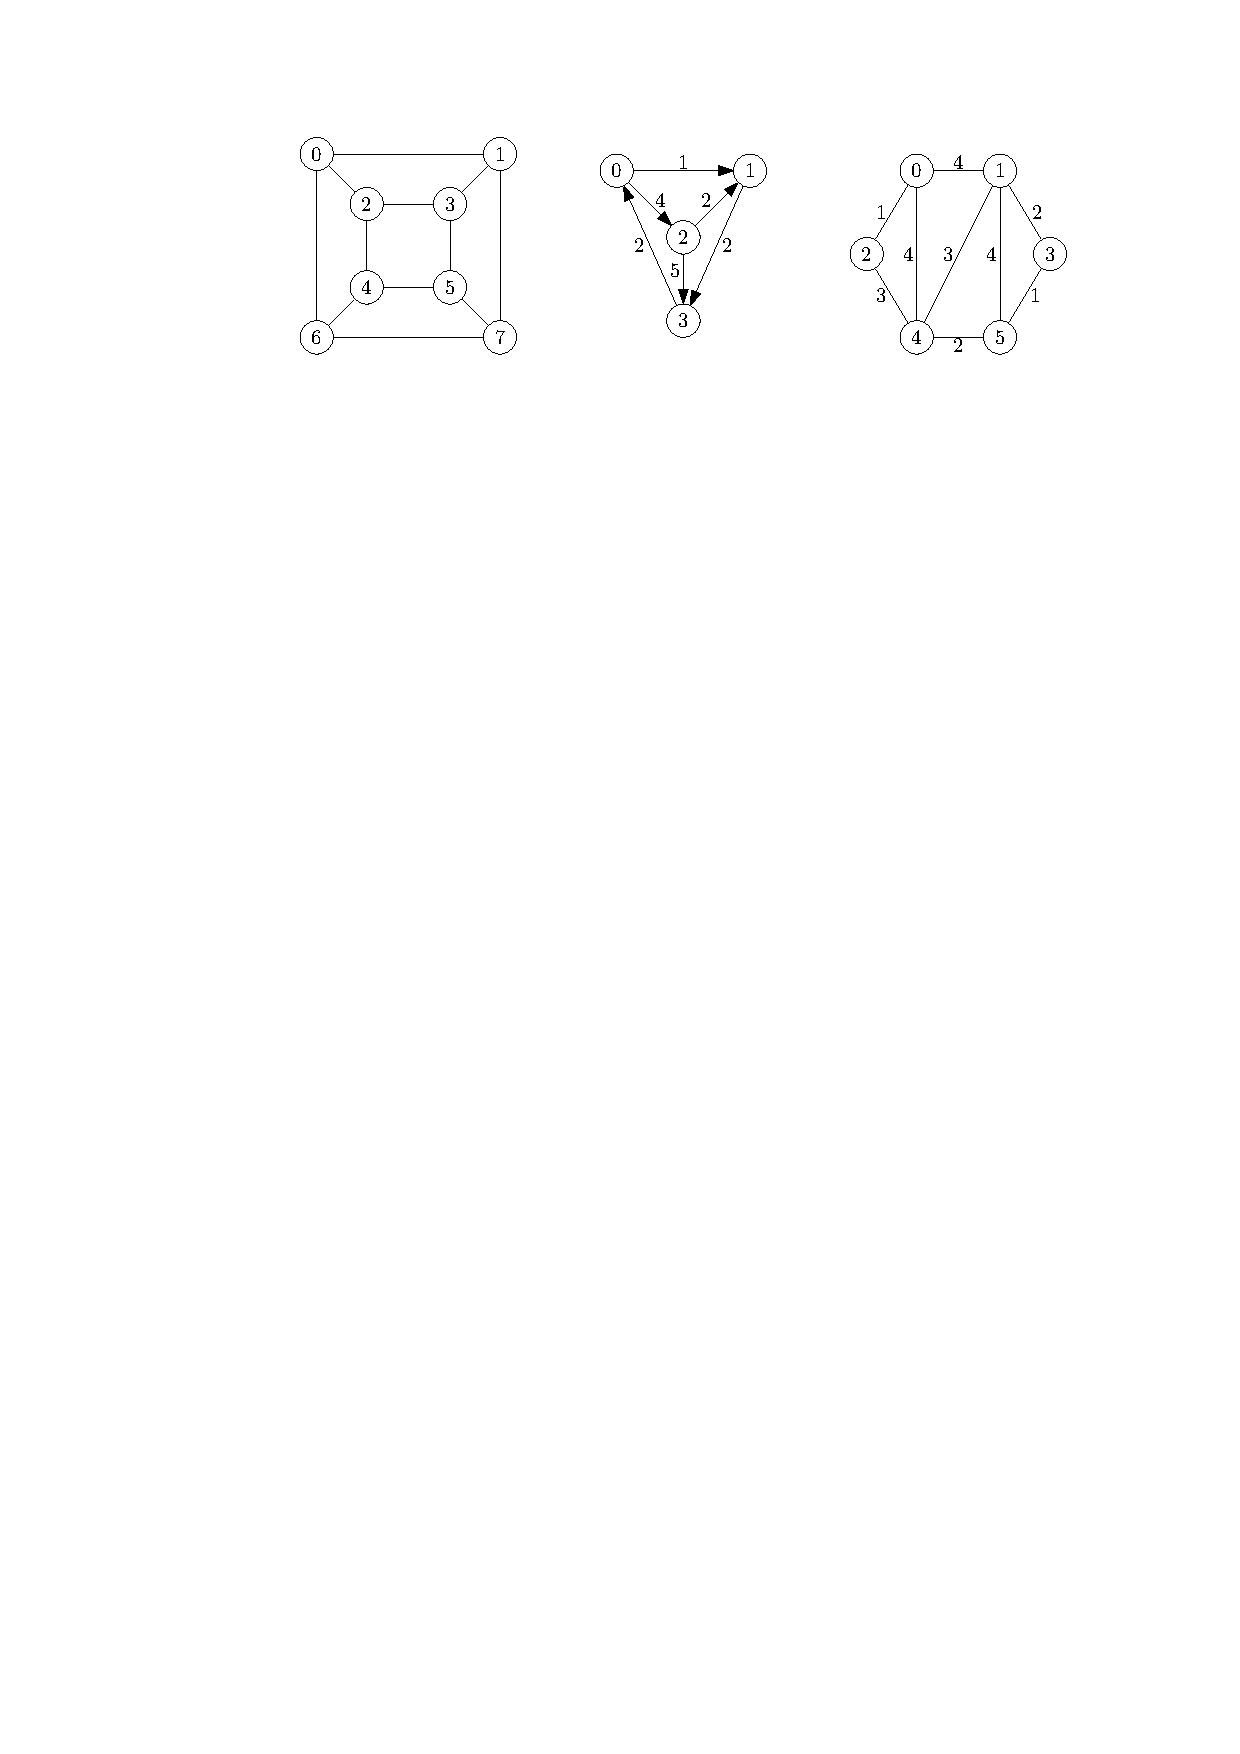
\includegraphics{graphExWeighted}
\end{center}
\end{Boxample}

Weighted digraphs can be represented using adjacency matrices or lists:
\begin{itemize}
  \item The adjacency matrix is modified so that each entry of $1$ (signifying that an arc exists) 
  is replaced by the cost of that arc.
  \item Care needs to be taken if using 0 to represent the absence of arcs, as 0 may be a legal edge weight. 
  In these cases, \texttt{null}, $\infty$ or some suitable value may be used.
  We use \boldfont{the convention that 0 or} \texttt{null} \textbf{represents the absence of an arc}. 
  \item An adjacency list is modified so that the list associated  with node $v$ has each adjacency node followed by the cost of the arc to the adjacent node. 
  \item For example, the list for node 6 with adjacent arcs $(6,2)$ with $c(6,2) = 4$ and $(6,7)$ with $c(6,7) = 5$ would be $2,4,7,5$.
\end{itemize}

\begin{Boxample}[0] \label{ex:drawWeightedGraph}
Draw the weighted graph given by the weighted matrix below. 
\newline

$\left[
\begin{array}{cccc}
	0 & 3 & 4 & 0  \\
	3 & 0 & 1 & 3  \\
	4 & 1 & 0 & 2  \\
	0 & 3 & 2 & 0  \\
\end{array}
\right]$
\vspace{1cm}


Draw the weighted digraph given by the weighted list representation below.
\newline

$\AdjLists{
\begin{tabular}{c|llll}
	0 & 1 & 3 & 2 & 4 \\
	1 & 0 & 2 & 3 & 2 \\
	2 & 1 & 3 &   &   \\
	3 & 2 & 1 &   &   \\
\end{tabular}
}$
\end{Boxample}


\section{Distance and diameter} \label{sec:unweighted}
Recall that the distance $d(u,v)$ between nodes $u$ and $v$ in an (unweighted) digraph 
is simply the number of arcs in the shortest path between them. 

In a weighted digraph, the distance to from node $u$ to $v$,  $d(u,v)$, is the cost of the minimum cost path from $u$ to $v$ where the cost of a path is just the sum of the costs on that path.


\begin{itemize}
  \item It is often helpful to have the \defnfont{distance matrix} for a digraph.
  The $(i, j)$-entry of this matrix contains the distance between node $i$ and node $j$.
  \item For an unweighted digraph, the distance matrix can be generated by running \texttt{BFSvisit}
  from each node in turn, since the distance to a node is equal to its depth in the BFS tree 
  (or infinite if the node is not reachable from the start node so not in the tree). 
  This gives an algorithm with running time in $\Theta(n^2 + nm)$.
\end{itemize}

\begin{Boxample}
A graph, its adjacency matrix and its distance matrix.\\

\begin{minipage}[c]{0.3\textwidth}
\centering
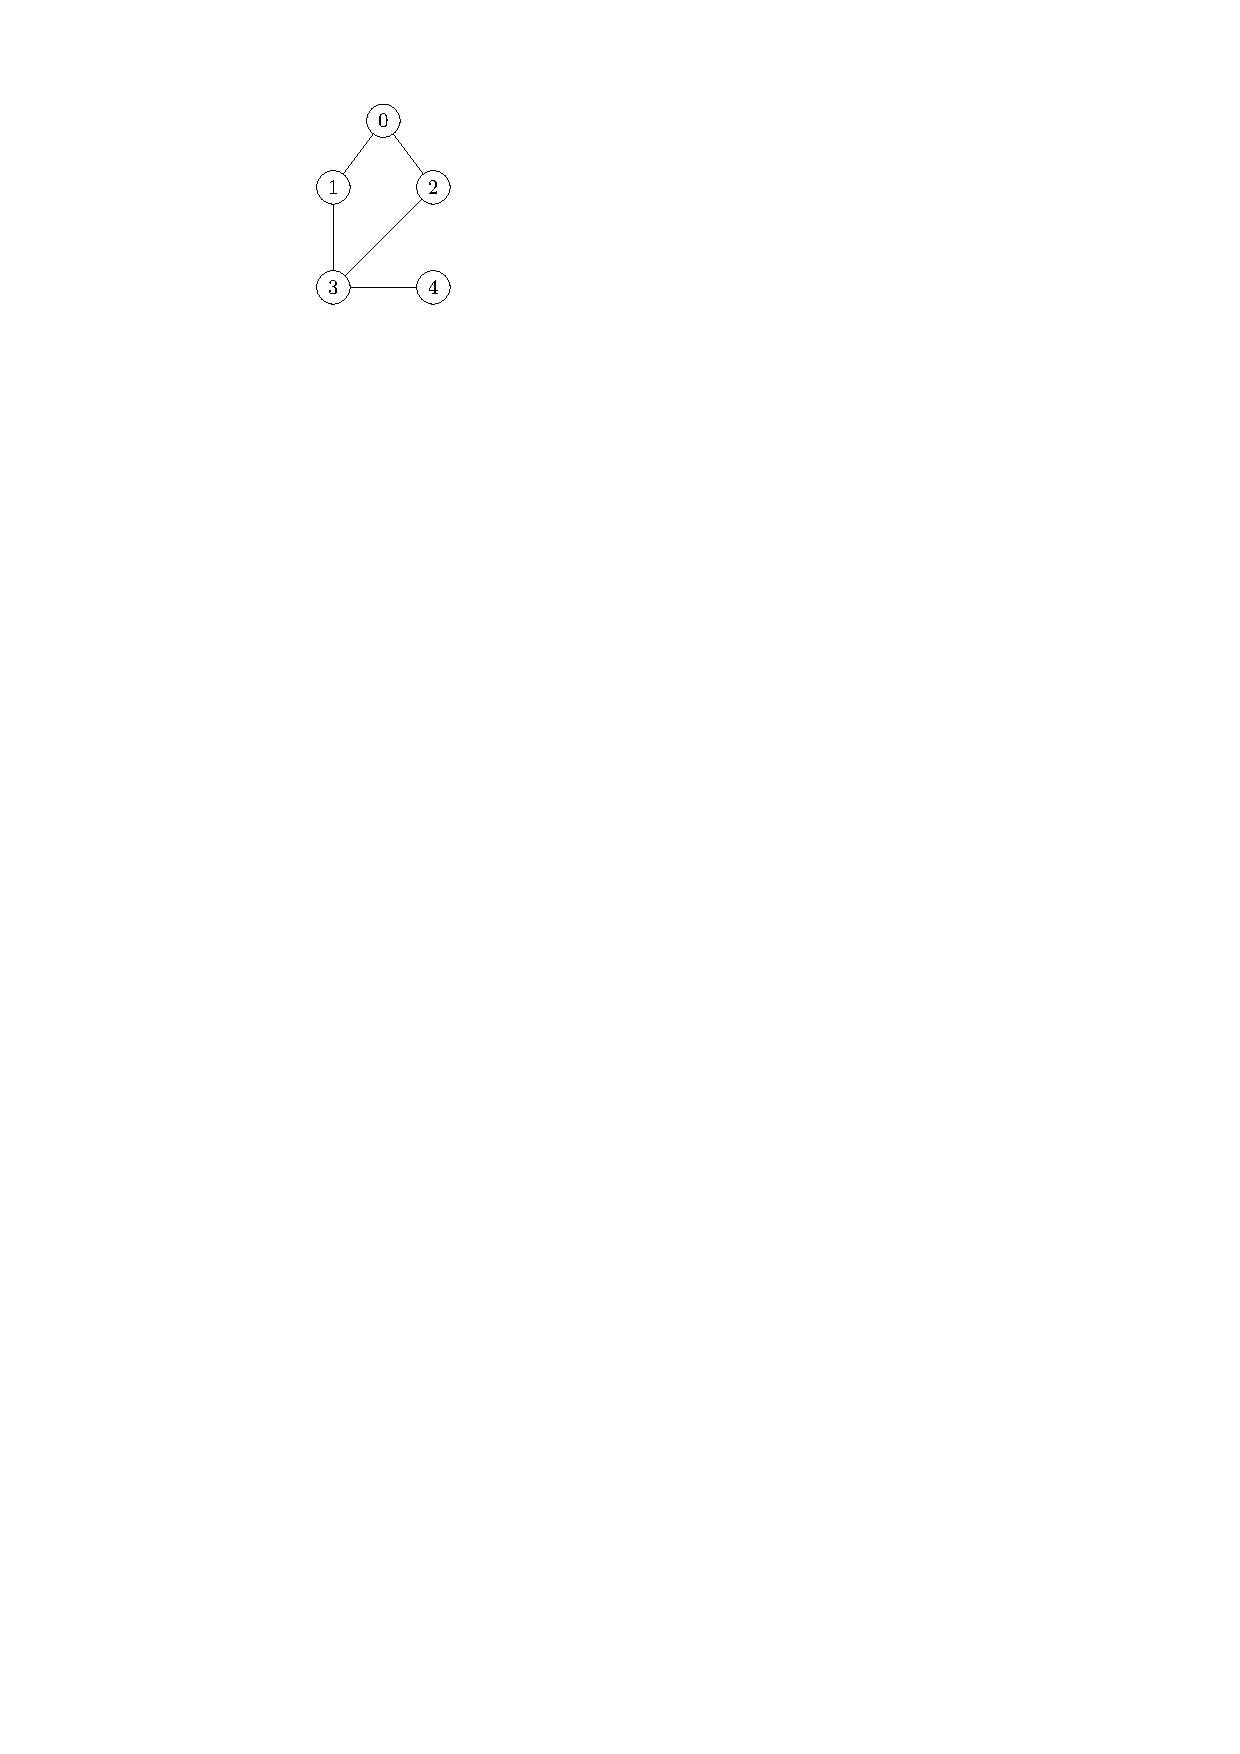
\includegraphics{distanceMatrixGraph}
\end{minipage}
\begin{minipage}[c]{0.65\textwidth}
$$\quad\left[
\begin{array}{ccccc}
0 & 1 & 1 & 0 & 0 \\
1 & 0 & 0 & 1 & 0 \\
1 & 0 & 0 & 1 & 0 \\
0 & 1 & 1 & 0 & 1 \\
0 & 0 & 0 & 1 & 0 \\
\end{array}
\right]
\hspace{1.5cm}
\left[
\begin{array}{ccccc}
0 & 1 & 1 & 2 & 3 \\
1 & 0 & 2 & 1 & 2 \\
1 & 2 & 0 & 1 & 2 \\
2 & 1 & 1 & 0 & 1 \\
3 & 2 & 2 & 1 & 0 \\
\end{array}
\right]$$
\end{minipage} 
\end{Boxample}

\begin{Boxample}[6]
Give an example of a weighted digraph in which the BFS approach
does not find the shortest path from the root to a node.
\end{Boxample}

\begin{Definition} \label{def:diameter}
The \defnfont{diameter} of a strongly connected digraph $G$ is the
maximum of $d(u,v)$ over all nodes $u, v \in V(G)$. 
If the digraph is not strongly connected the diameter is undefined though can be set to $\infty$.

\end{Definition}

 Clearly the diameter is just the maximum entry in the distance matrix.

\begin{Boxample}[1]
What is the diameter of the 3-cube in \cref{ex:graphExWeighted}?

\end{Boxample}

\section{Single-source shortest path problem} \label{sec:SSSP}
\begin{Definition}
In  the \defnfont{single-source shortest path problem} (SSSP) 
we are given a weighted digraph $(G, c)$ and a source node $s$. 
For each node $v$ of $G$, we must find the minimum weight of a path from $s$ to $v$.
By the weight of a path we mean the sum of the weights on the arcs. 
This is like finding row $s$ in a weighted distance matrix.
\end{Definition}

\begin{Boxample} \label{eg:SSSP}
In the weighted digraph pictured, the unique shortest path from $0$ to $3$ is $0, 1, 3$ with weight $3$.
What is the path with minimum weight from $2$ to $0$, and what is its weight?\\

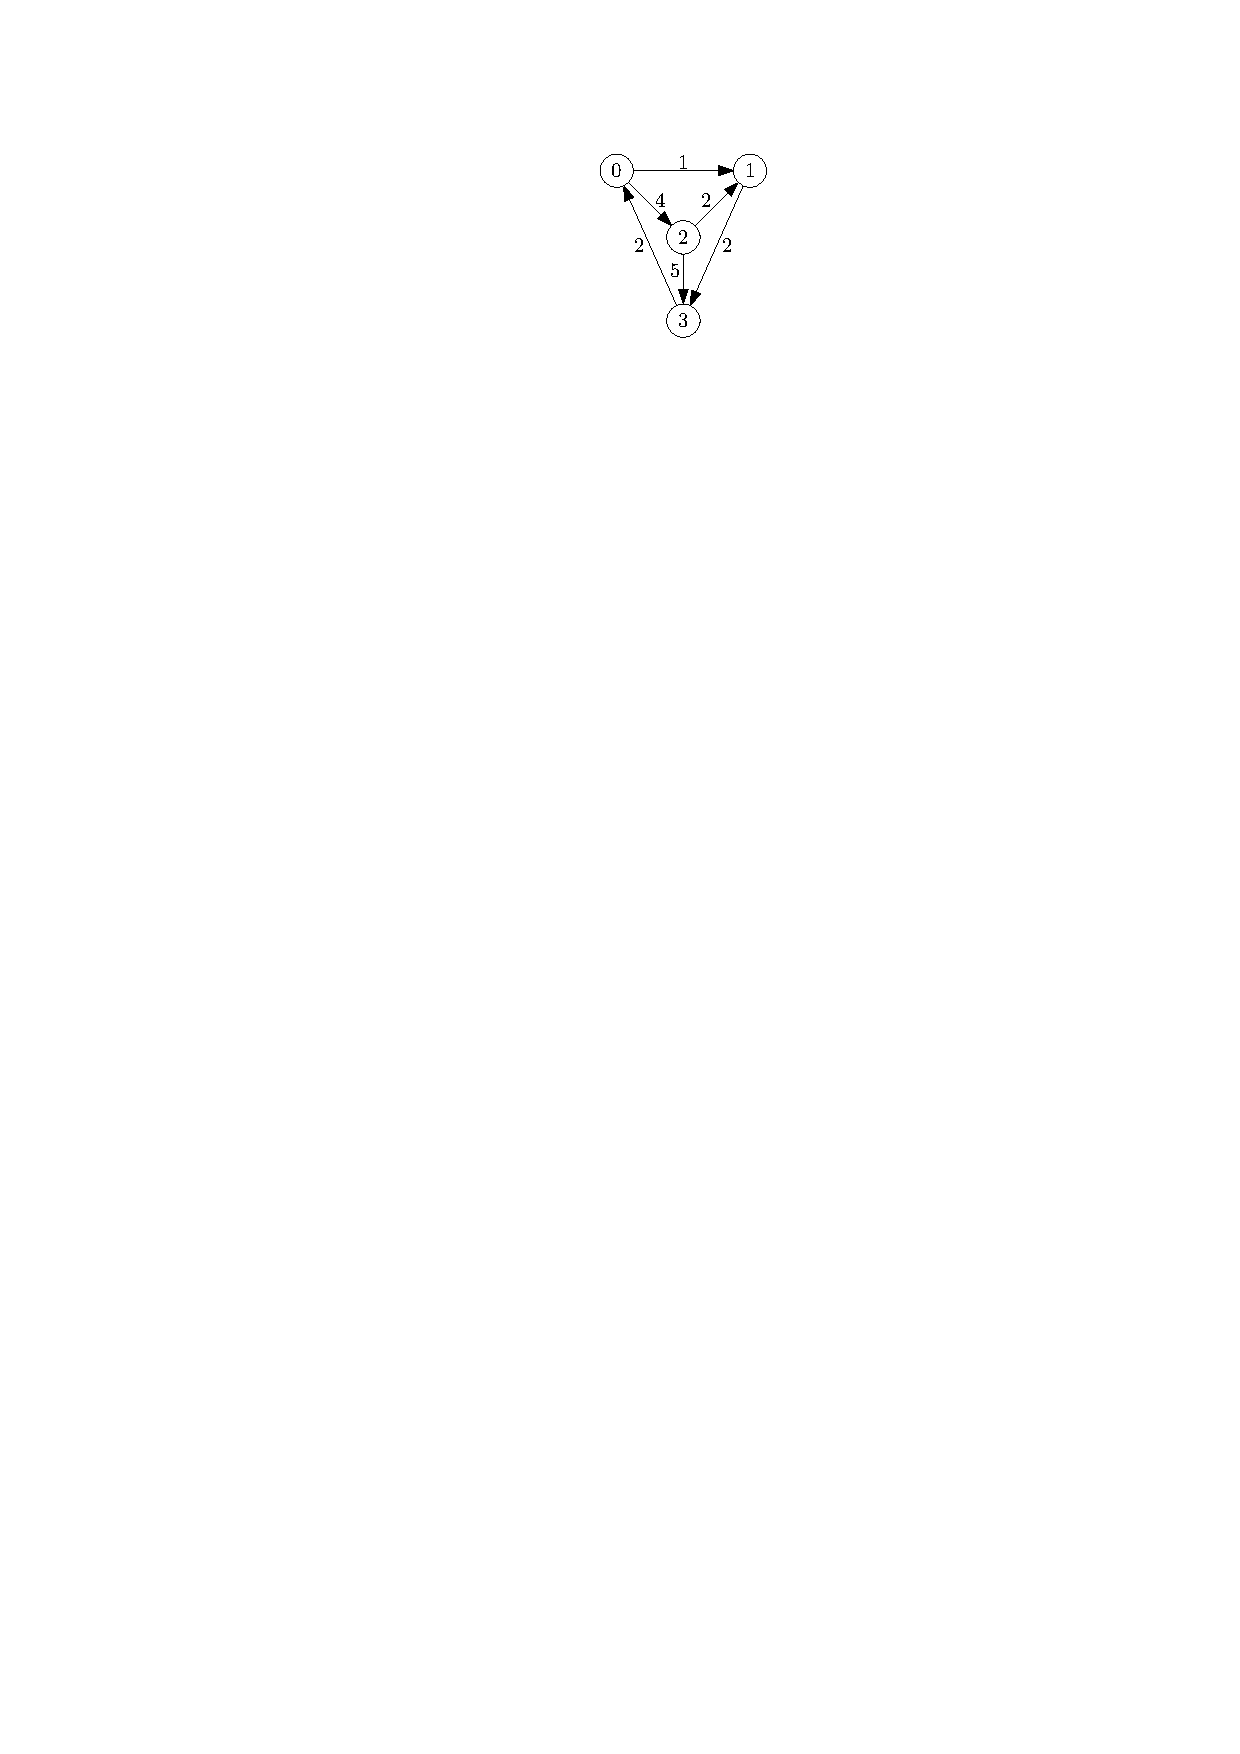
\includegraphics{weightedDigraph}
\end{Boxample}

\section{Dijkstra's algorithm}
\defnfont{Dijkstra's algorithm} solves the SSSP problem whenever \boldfont{all weights are non-\linebreak[4]negative}. 
It may fail in the presence of negative weight arcs.

It is easiest to understand the algorithm in terms of a set of visited nodes $S$, which eventually includes all nodes in $G$. 
We'll consider only shortest paths through $S$. % and make sure the length of these shortest paths is accurate.
Once $S = V(G)$, all shortest path lengths are known. 

Initially $S$ contains only the single node $s$. 
The only paths available are the one-arc paths from $s$ to neighbours $v$, of weight $c(s, v)$. 
We choose the neighbour $u$ with $c(s, u)$ minimal and add it to $S$. 

Now the fringe nodes adjacent to $s$ and $u$ must be updated to reflect possible paths through $u$ 
(it is possible that there exists a path from $s$ to $v$, passing through $u$, that is shorter than the direct path from $s$). 
Now we choose the node whose current best distance to $s$ is smallest, and update again. 
We continue in this way until all nodes belong to $S$. In \cref{alg:dijkstra}, the set $S$ consists of the BLACK nodes.

\begin{algorithm}[H]
  \caption{Dijkstra's algorithm, first version.}
    \label{alg:dijkstra}
\begin{algorithmic}[1]
\Function{Dijkstra}{weighted digraph $(G, c)$; node $s \in V(G)$}
	\State array $\colour[0..n-1]$, $\dist[0..n-1]$
	\For{$u \in V(G)$}
		\State $\dist[u] \gets c[s,u]$; $\colour[u] \gets$ WHITE 
	\EndFor
	\State $\dist[s] \gets 0$; $\colour[s] \gets $ BLACK
	\While{there is a white node}
		\State find a white node $u$ so that $\dist[u]$ is minimum
		\State $\colour[u] \gets $ BLACK
		\For{$x \in V(G)$}
			\If{$\colour[x] = $ WHITE}
				\State $\dist[x] \gets \min \{\dist[x], \dist[u] + c[u,x]\}$  
			\EndIf
		\EndFor
	\EndWhile
	\State \Return{$\dist$}
\EndFunction
\end{algorithmic}
\end{algorithm}

\begin{Boxample}
An application of Dijkstra's algorithm with starting vertex $0$. 
The distances to 0 at each step are displayed next to each node.
\begin{center}
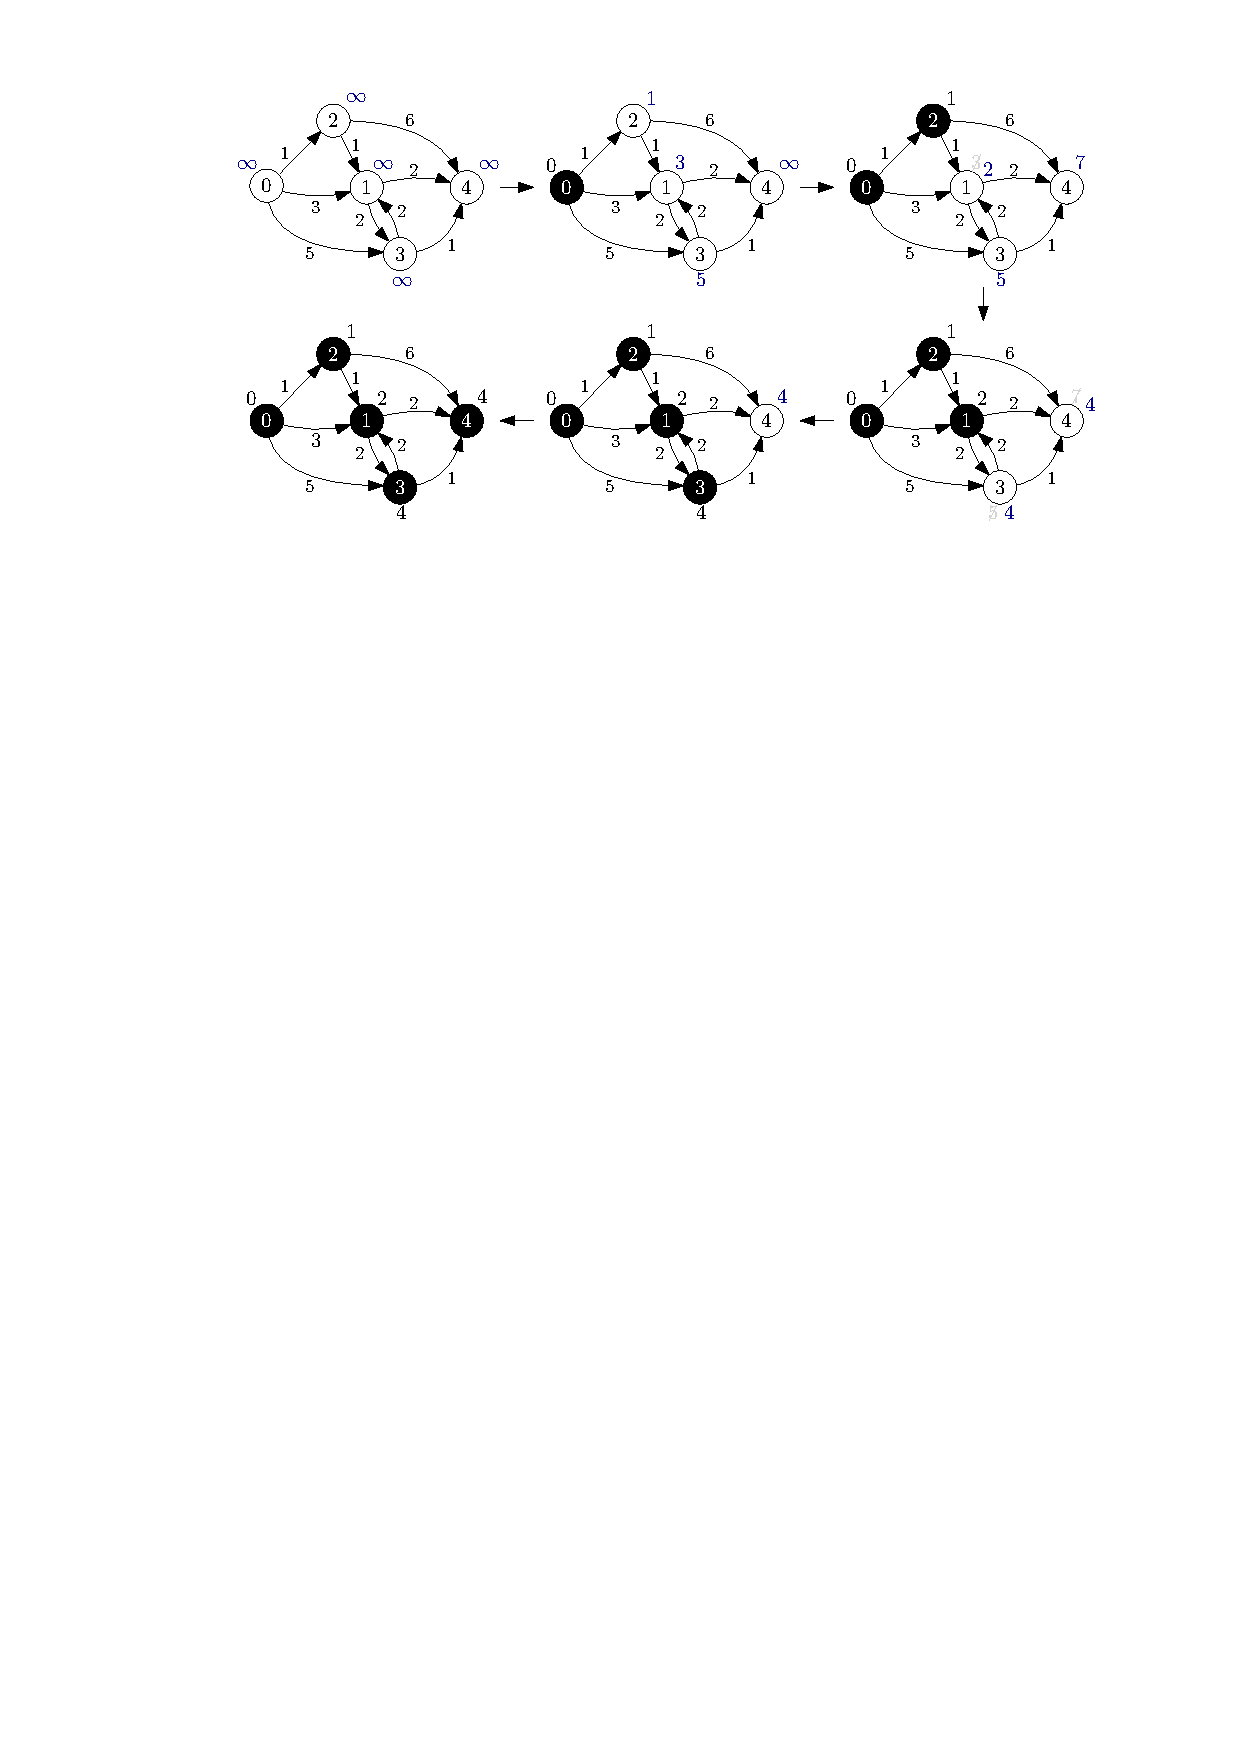
\includegraphics[width=1.0\textwidth]{DijkstraEx2}
\end{center}
\end{Boxample}

Dijkstra's algorithm is an example of a \defnfont{greedy algorithm}. 
At each step it makes the best choice involving only local information,
and never regrets its past choices. 

\begin{Boxample}\mbox{}\\
  \label{ex:dijs-all-vert}
  \begin{minipage}[c]{0.45\textwidth}
	An application of Dijkstra's algorithm on the digraph below
	for each starting vertex $s$. 
	Complete the table for the starting vertex 2.
	
	\begin{center}
	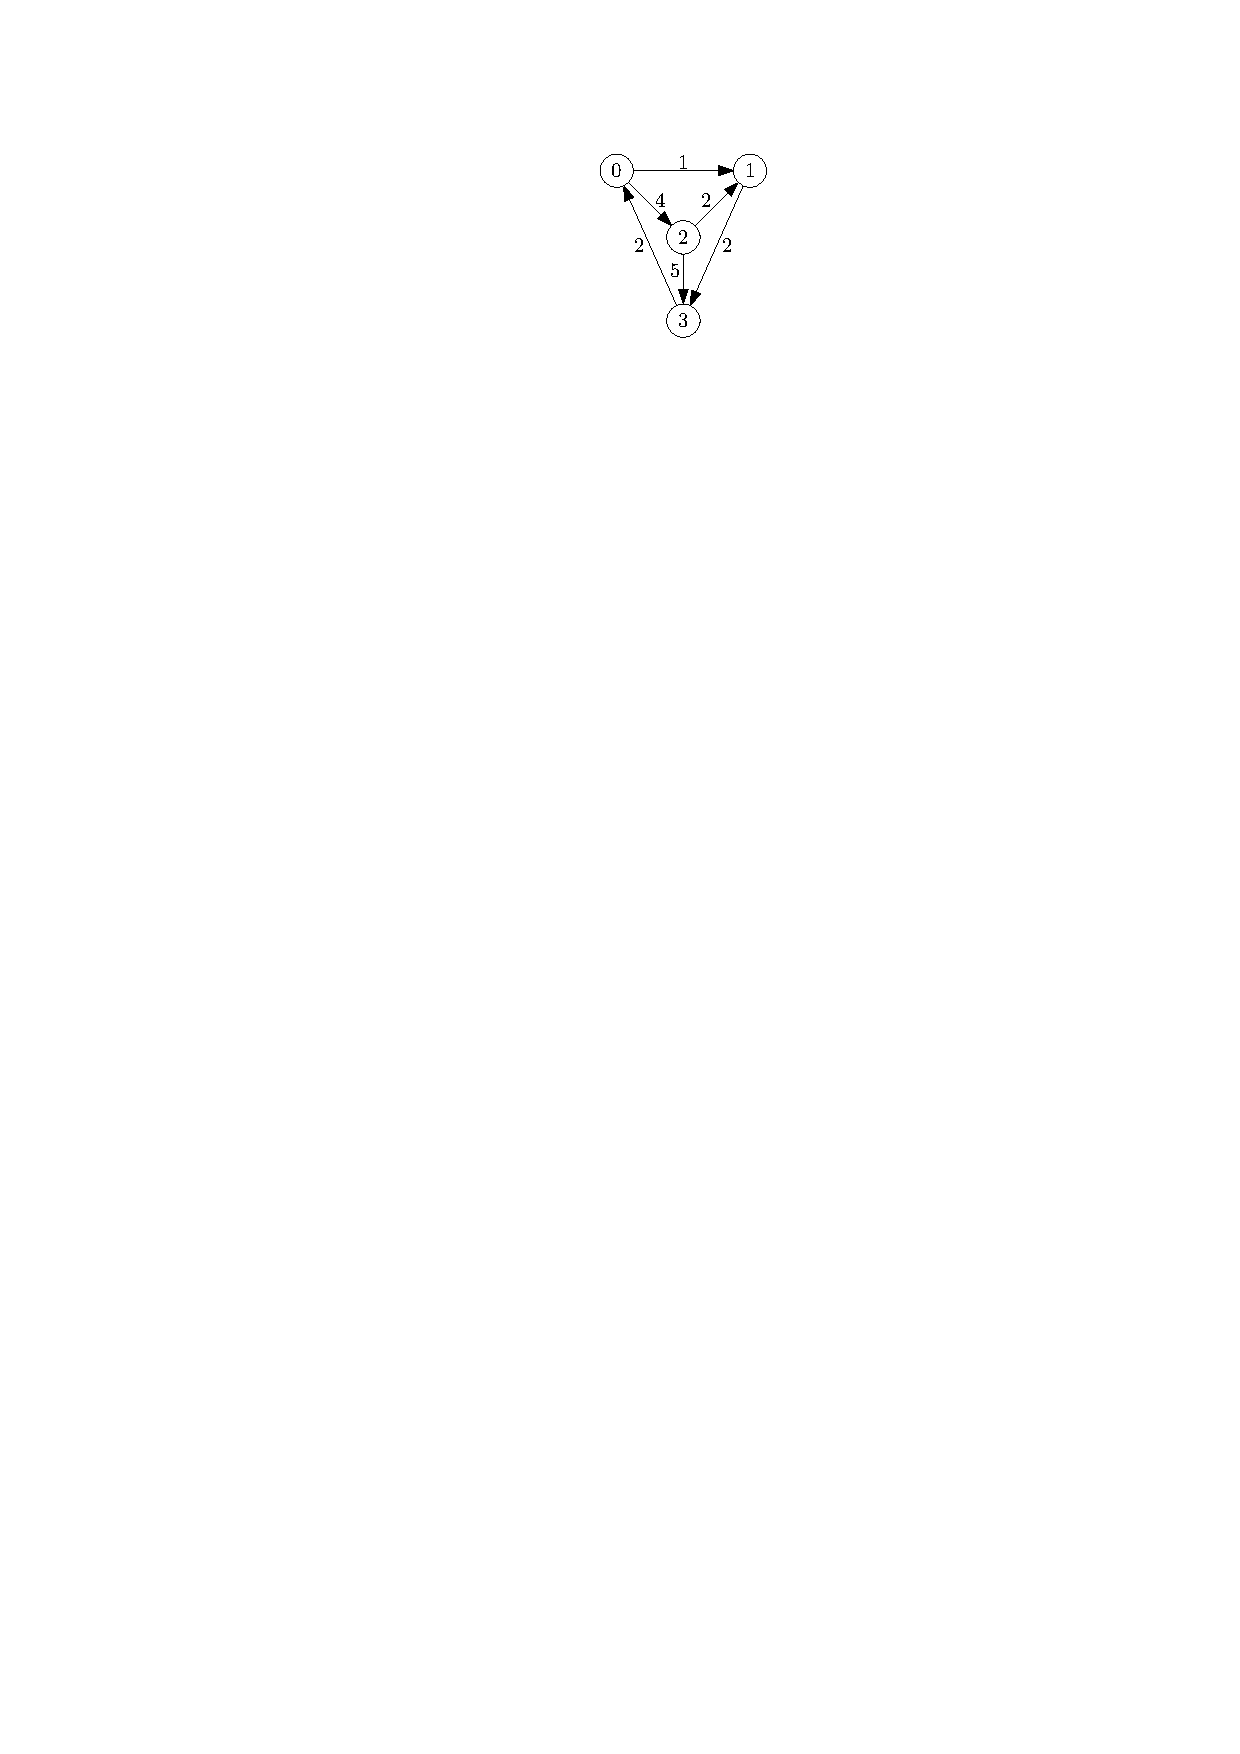
\includegraphics{weightedDigraph}
	\end{center}
	
	The table illustrates that the distance vector is updated at 
	most $n - 1$ times (only before a new vertex is selected and added to $S$). 
	Thus we could have omitted the lines with $S = \set{0,1,2,3}$.
  \end{minipage}$\quad$
  \begin{minipage}[c]{0.45\textwidth}
	\begin{tabular}{|c|c|}\hline
		\textbf{current} $S \subseteq V$ &  \textbf{distance vector} $\dist$ \\ \hline
		\set{0}       & $0, 1, 4, \infty$  \\
		\set{0,1}     & $0, 1, 4, 3$  \\
		\set{0,1,3}   & $0, 1, 4, 3$  \\
		\set{0,1,2,3} & $0, 1, 4, 3$  \\ 
			\hline
		\set{1}       & $\infty, 0, \infty, 2$  \\
		\set{1,3}     & $4, 0, \infty, 2$ \\
		\set{0,1,3}   & $4, 0, 8, 2$ \\
		\set{0,1,2,3} & $4, 0, 8, 2$ \\ 
		\hline
		\set{2}           & \\%$\infty, 2, 0, 5$  \\
		&\\
		\set{\qquad}      & \\%$\infty, 2 , 0, 4$ \\
		&\\
		\set{\qquad\quad} & \\%$6, 2, 0, 4$  \\
		&\\
		\set{0,1,2,3}     & \\ %\hline %$6, 2, 0, 4$ \\ \hline
		&\\ \hline
		\set{3}       & $2, \infty, \infty, 0$ \\
		\set{0,3}     & $2, 3, 6, 0$ \\
		\set{0,1,3}   & $2, 3, 6, 0 $ \\
		\set{0,1,2,3} & $2, 3, 6, 0$ \\ \hline
	\end{tabular}
  \end{minipage}\\
\end{Boxample}


\chapter{Dijkstra proof and running time} %--------------------------------------
\begin{Boxample}[0.5] \label{ex:dijk-neg-fails}
Give weights to the edges of the digraph below so that running Dijkstra's algorithm 
with starting vertex $0$ fails. 
\vspace{0.5cm} 
\begin{center}
  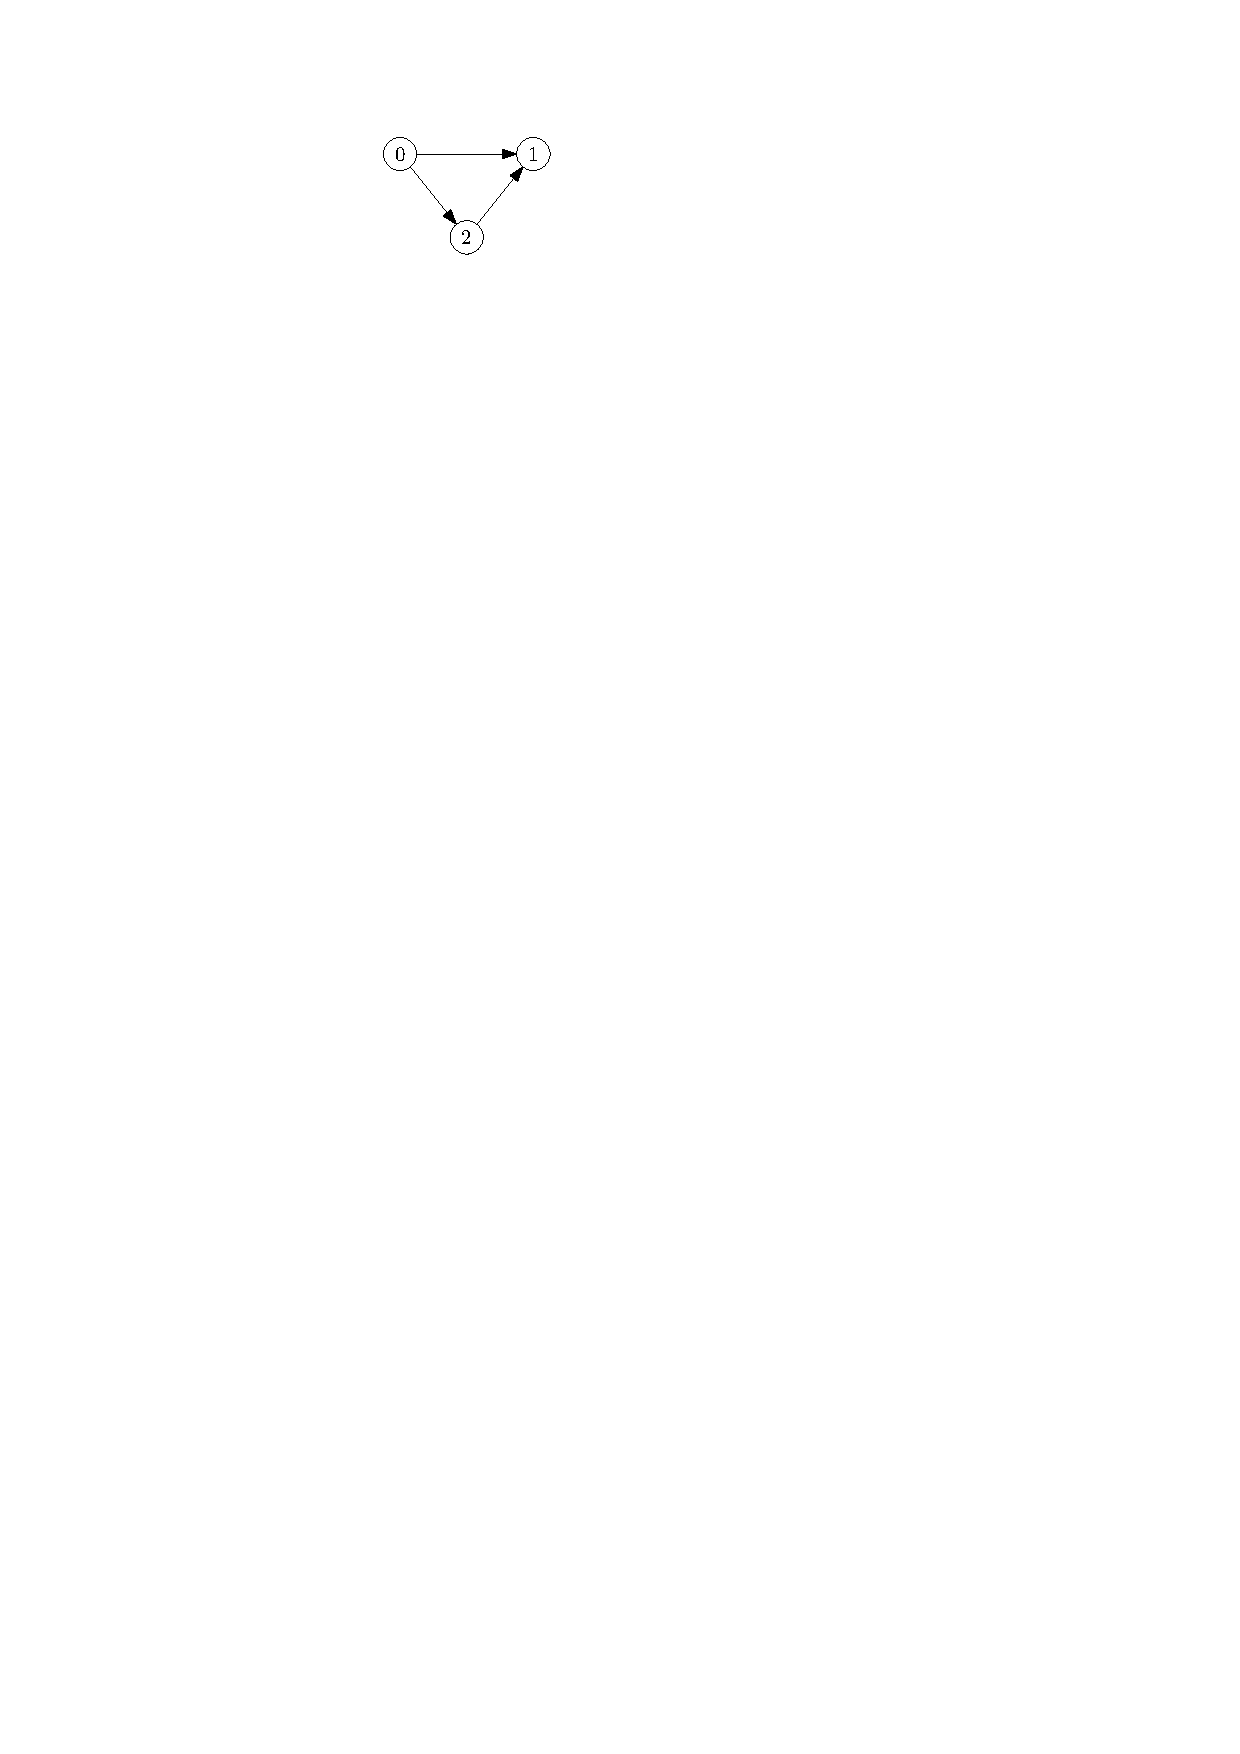
\includegraphics{DijkstraTriangle}
\end{center}
\end{Boxample}

Proving Dijkstra's algorithm works is trickier than for other algorithms we've seen.

Define an \defnfont{$\boldsymbol S$-path} from $s$ to $w$ as a
path from $s$ to $w$ with $s$ and all intermediate nodes belonging to $S$. 
In other words, $w$ may not belong to $S$, but all other nodes in the path do.

\begin{Theorem}
\label{thm:dijkstra} Suppose that all arc weights are non-negative. 
Then at the top of the \boldfont{while} loop, we have the following properties:
\begin{description}
  \item[P1:] If $x \in V(G)$, then $\dist[x]$ is the minimum cost of an $S$-path from $s$ to $x$.
  \item[P2:] If $w \in S$, then $\dist[w]$ is the minimum cost of a path from $s$ to $w$.
\end{description}
\end{Theorem}
%\begin{proof} 
At every step, $\dist[x]$ is the length of some path from $s$ to $x$, or $\infty$. 
That path is an $S$-path if $x \in S$. 
Also note that the update formula ensures that $\dist[x]$ never increases. 

To prove P1 and P2, we use induction on the number of times $k$ we
have been through the while-loop. Let $S_k$ denote the value of $S$
at this stage. 

\begin{Boxample}[3]
Show that P1 and P2 hold when $k = 0$.
\end{Boxample}
\begin{Boxample}[9]
Show that P1 holds for any value of $k$.
\end{Boxample}
\begin{Boxample}[9]
Show that P2 holds for any value of $k$ and that this proves the correctness of Dijkstra's algorithm.
\end{Boxample}
%
%To prove P1 and P2, we use induction on the number of times $k$ we
%have been through the while-loop. Let $S_k$ denote the value of $S$
%at this stage. 
%When $k = 0$, $S_0 = \{s\}$, and since $\dist[s] = 0$, P1 and P2 obviously hold. 
%Now suppose that they hold after $k$ times through the while-loop 
%and let $u$ be the next special node chosen during that loop. 
%Thus $S_{k+1} = S_k \cup \set{u}$.
%
%We first show that P2 holds after $k + 1$ iterations.
%If $x \in S$, P2 trivially holds for $x$ by the inductive hypothesis. 
%For $x = u$, suppose for the sake of contradiction that there is a shortest path $\gamma$ from $s$ to $u$ 
%that is not an $S_{k+1}$-path.
%Then $\gamma$ contains a vertex $y$ not in $S_{k}$ with a smaller distance to $s$ than $u$. 
%However, then $y$ would have been picked prior to $u$.
%Hence, no such path $\gamma$ can exist and P2 holds for every iteration.

%Next we show that P1 holds after $k + 1$ iterations.
%For $x \in S_k$, P1 holds by the inductive hypothesis.
%It holds for $x = u$, since otherwise $u$ would have been picked earlier.
%For $x \not \in S_{k+1}$, it follows from the inductive hypothesis, the choice of $u$, and the update formula that P1 holds. 
%Hence P1 holds for all iterations.
%\end{proof}

%That P2 also holds after the last iteration proves the correctness of Dijkstra's algorithm.

\section{Running time of Dijkstra}
%The study of the time complexity of Dijkstra's algorithm leads to many interesting topics.

The value of $\dist[x]$ will change only if $x$ is adjacent to $u$.
Thus if we use a weighted adjacency list, the block inside the
second for-loop need only be executed $m$ times. 
However, if using the adjacency matrix representation, the block inside the for-loop
must still be executed $n^2$ times.

The time complexity is of order $a n + m$ if adjacency lists are used,
and $a n + n^2$ with an adjacency matrix, where $a$ represents the time
taken to find the node with minimum value of $\dist$. 
The obvious method of finding the minimum is simply to scan through array $\dist$
sequentially, so that $a$ is of order $n$, and the running time of
Dijkstra is therefore $\Theta(n^2)$. 
%Dijkstra himself originally used an adjacency matrix and scanning of the $\dist$ array. 

The next lecture looks at a more efficient implementation with running time $O((m+n)\log n)$.

\chapter{Dijkstra and PFS, Bellman-Ford algorithm} % -----------------------------------

\section{PFS implementation of Dijkstra}
\begin{itemize}
  \item We can implement Dijkstra's algorithm using priority-first search ideas. 
  \item The key value associated to a node $u$ is simply the value $\dist[u]$,
  the current best distance to that node from the root $s$.
\end{itemize}

\begin{algorithm}[H]
  \caption{Dijkstra's algorithm, PFS version.}
  \label{alg:dijkstra2}
\begin{algorithmic}[1]
\Function{Dijkstra2}{weighted digraph $(G, c)$; node $s \in V(G)$}
	\State priority queue $Q$
	\State array $\colour[0..n-1]$, $\dist[0..n-1]$
	\For{$u \in V(G)$}
		\State $\colour[u] \gets$ WHITE 
	\EndFor
	\State $\colour[s] \gets $ GREY
	\State $Q$.\texttt{insert}$(s, 0)$
	\While{\textbf{not} $Q$.\texttt{isEmpty}$()$}
		\State $t_1 \gets$  $Q$.\texttt{getKey}$Q$.\texttt{peek}$()$
		\State $u \gets Q$.\texttt{pop}$()$
		\For{each $x$ adjacent to $u$}
			\State $t_2 \gets t_1 + c(u, x)$
			\If{$\colour[x] = $ WHITE}
				\State $\colour[x] \gets $ GREY
				\State $Q$.\texttt{insert}$(x, t_2)$
			\ElsIf{$\colour[x] = $ GREY \textbf{and} $Q$.\texttt{getKey}$(x) > t_2$}
				\State $Q$.\texttt{decreaseKey}$(x, t_2)$
			\EndIf
		\EndFor
		\State $\colour[u] \gets $ BLACK
		\State $\dist[u] \gets t_1$ 
	\EndWhile
	\State \Return{$\dist$}
\EndFunction
\end{algorithmic}
\end{algorithm}


We can see that the dominant operations in terms of running time are 
\begin{itemize}
\item $n$ delete-min operations, and
\item  (at most) $m$ decrease-key operations. 
\end{itemize}
Hence using a binary heap, Dijkstra's
algorithm runs in time $O((n + m) \log n)$. 
Thus if every node is reachable from the source, it runs in time $O(m \log n)$.

%Specialised data structures to implement priority queues can improve the running time of Dijktra's.
The best complexity bound for Dijkstra's algorithm, using a \boldfont{Fibonacci heap}, is $O(m + n\log n)$.

\section{Bellman--Ford algorithm} \label{sec:bellford}
The \defnfont{Bellman--Ford algorithm} solves the SSSP problem \boldfont{even when there are negative weight arcs}. 
It is not surprising that the algorithm thus runs more slowly than Dijkstra's algorithm. 
\begin{itemize}
  \item The basic idea, as with Dijkstra's algorithm, is to solve the SSSP under restrictions that become progressively more relaxed. 
  \item Bellman--Ford solves the problem for all nodes at ``level" $0, 1, \dots , n-1$ in turn.
  \item By level we mean the minimum possible number of arcs in a minimum weight path to that node from the source.
\end{itemize}

\begin{algorithm}[H]
  \caption{Bellman--Ford algorithm.}
  \label{alg:bellford-code}
\begin{algorithmic}[1]
\Function{BellmanFord}{weighted digraph $(G, c)$; node $s \in V(G)$}
	\State array $\dist[0..n-1]$
	\For{$u \in V(G)$}
		\State $\dist[u] \gets \infty$ 
	\EndFor
	\State $\dist[s] \gets 0$
	\For{$i$ \textbf{from} $0$ \textbf{to} $n-1$}
		\For{$x \in V(G)$}
			\For{$v \in V(G)$}
				\State $\dist[v] \gets \min( \dist[v], \dist[x] + c(x,v) )$
			\EndFor
		\EndFor
	\EndFor
	\State \Return{$\dist$}
\EndFunction
\end{algorithmic}
\end{algorithm}

\begin{Boxample}[0]
An application of Bellman--Ford algorithm with starting node $4$
when the nodes are processed in the order from $0$ to $4$.
\begin{center} 
  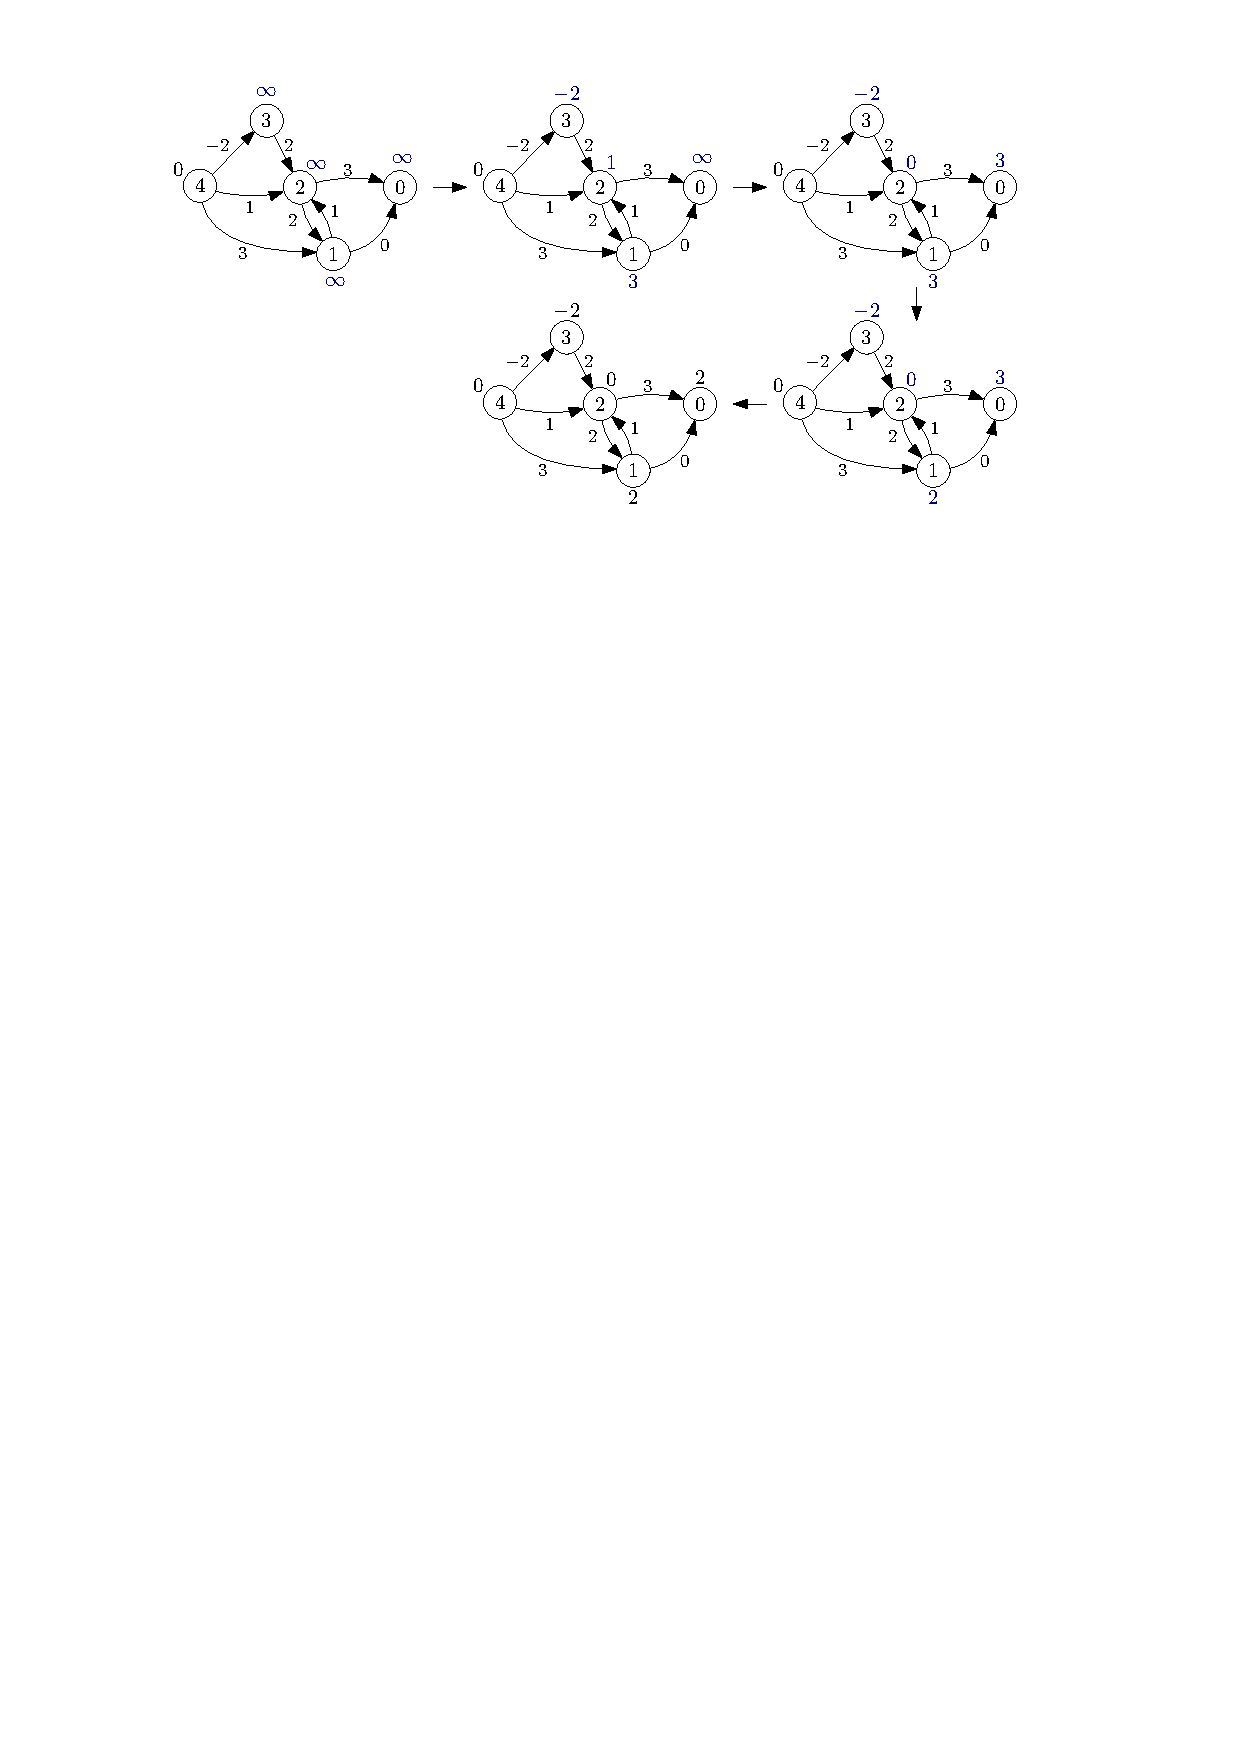
\includegraphics[width=1.0\textwidth]{BellmanFordEx2}
\end{center}
%After how many iterations would the algorithm converge to the exact distance, 
%if the nodes are processed in the order $4$, $3$, $2$, $1$, $0$?
\end{Boxample}

\begin{Boxample}[0]
Execute the Bellman--Ford algorithm on the graph below with starting vertex $0$.
Process nodes in the order from $0$ to $5$.
\begin{center} 
  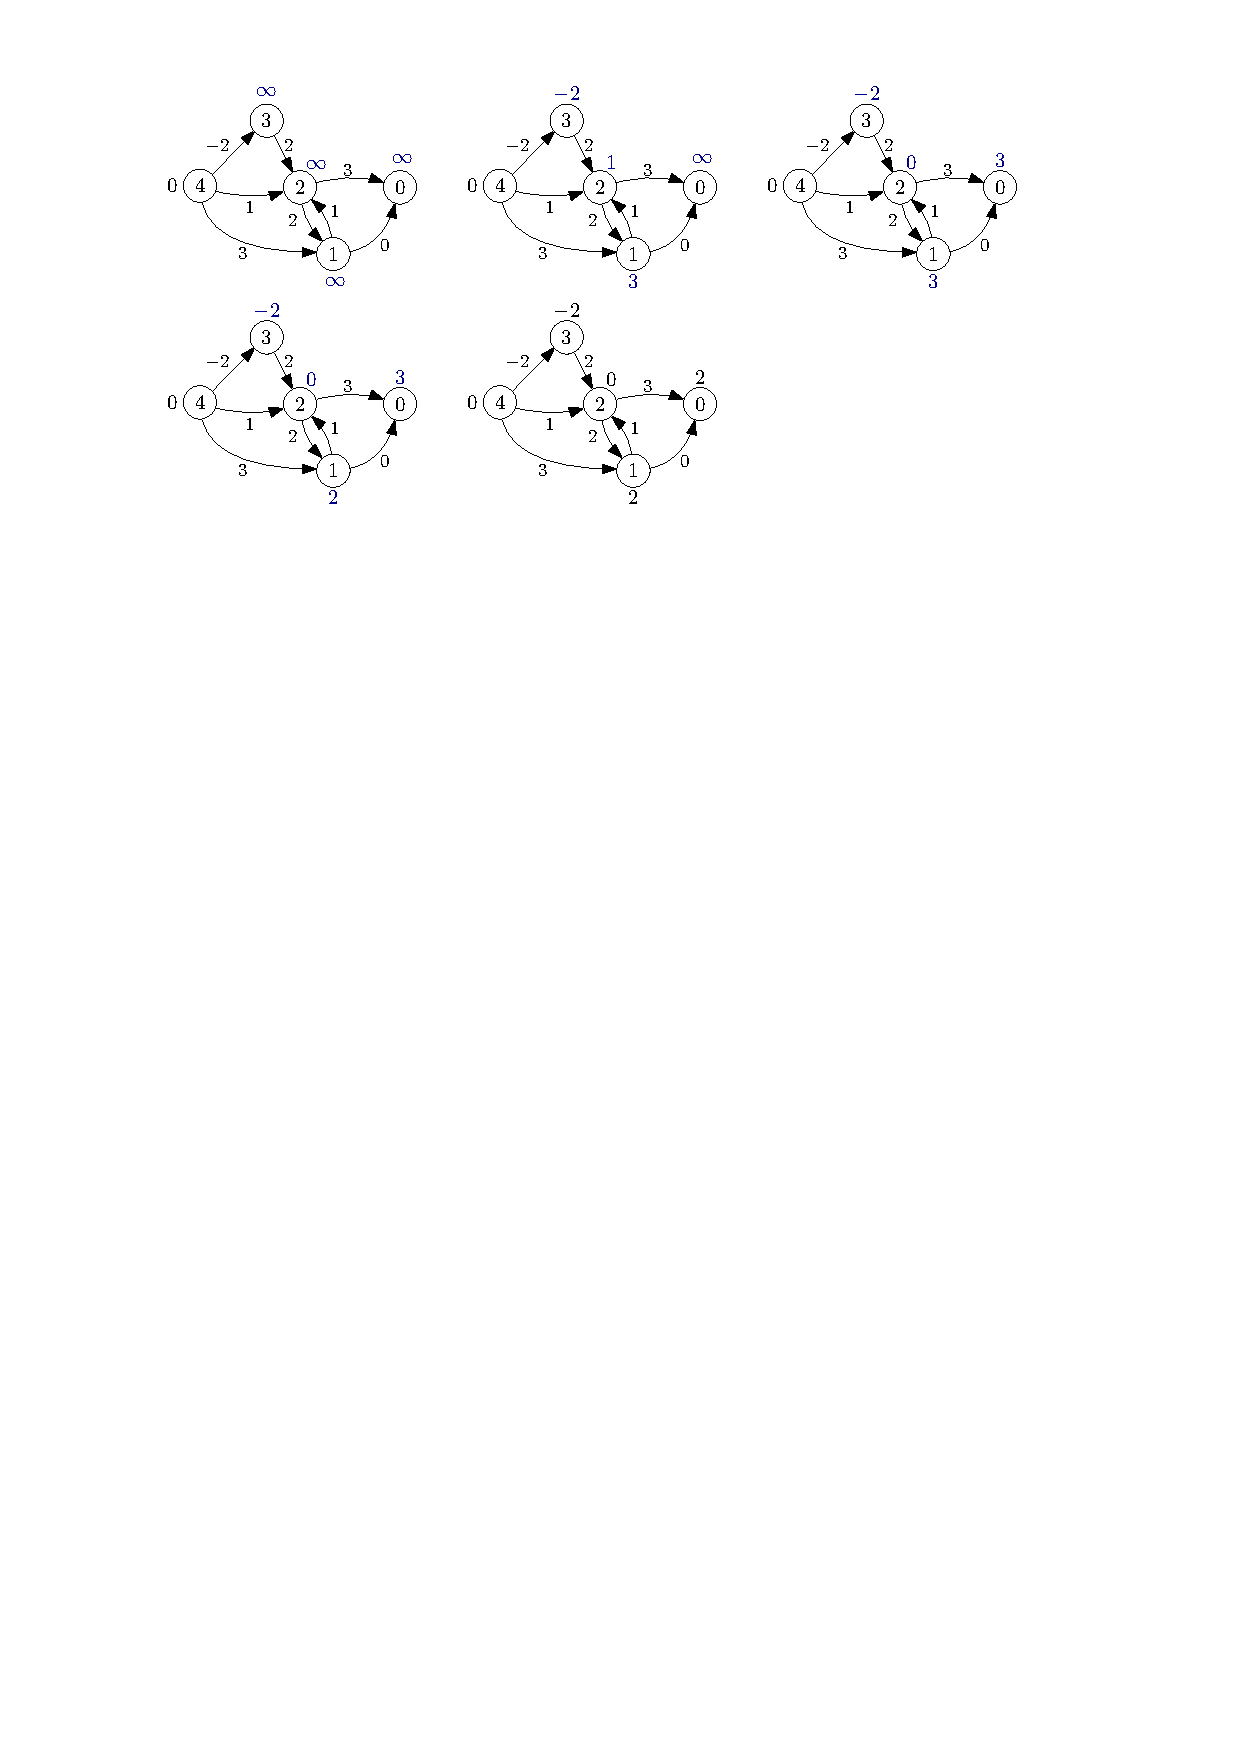
\includegraphics[width=1.0\textwidth]{BellmanFordEx}
\end{center}
\end{Boxample}


\begin{Theorem} 
Suppose that $G$ contains no negative weight cycles. Then after the $i$-th 
iteration of the outer for-loop, $\dist[v]$ contains the minimum weight of a 
path to $v$ for all nodes $v$ with level at most $i$.
\end{Theorem}
\begin{proof} 
Note that as for Dijkstra, the update formula is such that $\dist$ values never increase.

We use induction on $i$. When $i=0$ the result is true because of our
initialization. Suppose it is true for $i-1$. Let $v$ be a node at level
$i$, and let $\gamma$ be a minimum weight path from $s$ to $v$. Since
there are no negative weight cycles, $\gamma$ has $i$ arcs. If $y$
is the last node of $\gamma$ before $v$, and $\gamma_1$ the subpath to
$y$, then by the inductive hypothesis we have $\dist[y] \leq | \gamma_1
|$. Thus by the update formula we have $\dist[v] \leq \dist[y] + c(y, v)
\leq | \gamma_1 | + c(y, v) \leq | \gamma |$ as required.
\end{proof}

The Bellman--Ford algorithm runs in time $\Theta(nm)$ using adjacency
lists, since the statement in the inner for-loop need only be
executed if $v$ is adjacent to $x$, and the outer loop runs $n$
times. Using an adjacency matrix it runs in time $\Theta(n^3)$.

\begin{Boxample}[2] \label{ex:SSSP-neg-cycle}
Explain why the SSSP problem makes no sense if we allow digraphs with
cycles of negative total weight.
\end{Boxample}

% \begin{Boxample} \label{ex:dijk-SI} % maybe use for assignment (on North Island)?
% The graph shows minimum legal driving times (in multiples of 5 minutes) 
% between various South Island towns. What is the shortest time to drive legally from
% Picton to (a) Wanaka, (b) Queenstown and (c) Invercargill? Explain which
% algorithm you use and show your work.
% \begin{center}
% 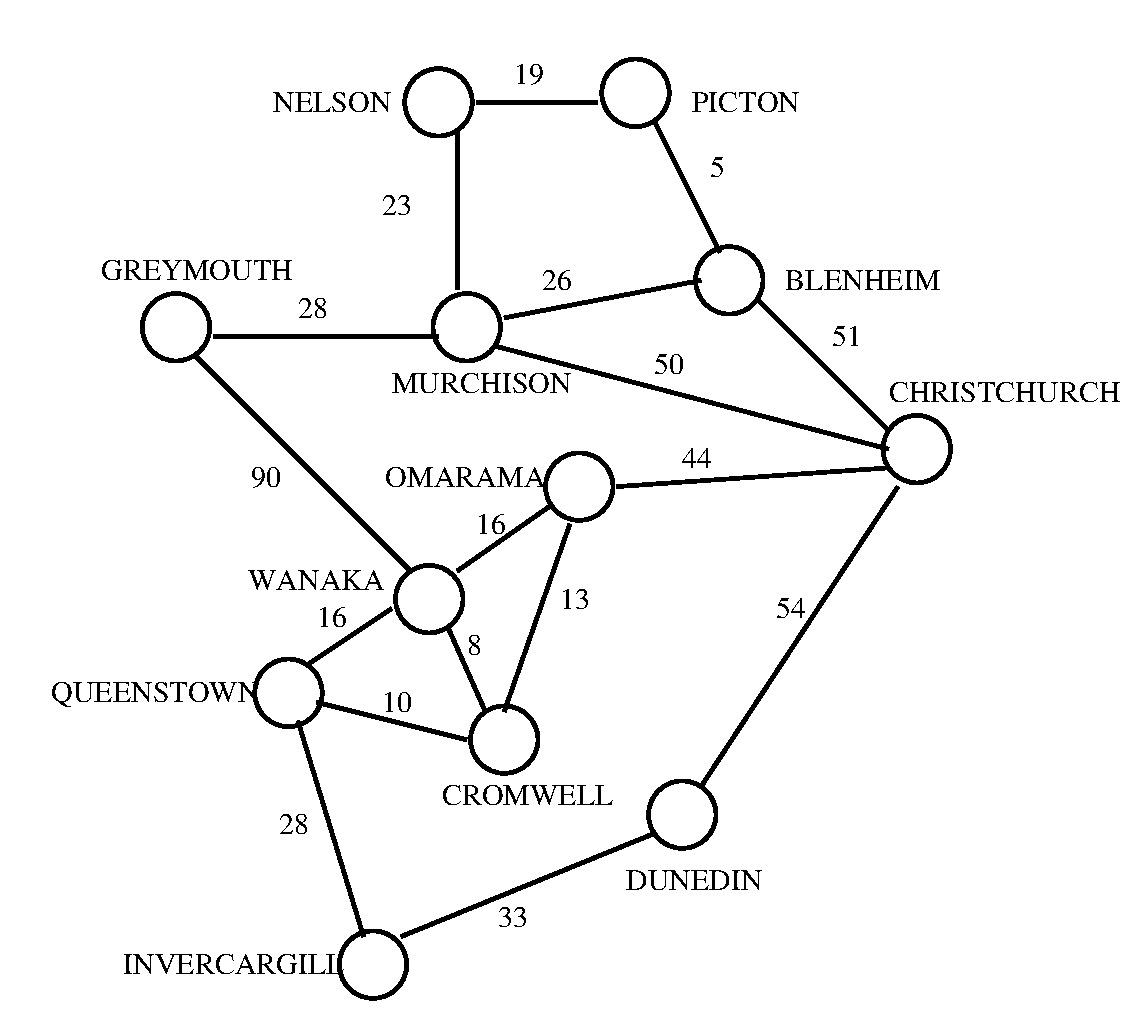
\includegraphics[width=8cm]{southisland}
% %\verb|\epsfig{figure=figs/SI.xfg.eps, width=12cm}|
% \end{center}
% \end{Boxample}

\begin{Boxample}[4]\label{ex:bellman-neg-cycle}
Suppose the input to the Bellman--Ford algorithm is a digraph with a
negative weight cycle. How could the algorithm detect this, so it can
exit gracefully with an error message?
\end{Boxample}


% \begin{Boxample}  \label{ex:dijk-proof}
% Where in the proof of Dijkstra's algorithm do we use the fact that 
% all the arc weights are non-negative?
% \end{Boxample}


\chapter{All-pairs shortest path problem} %-----------------------------------
\label{sec:APSP}

\begin{Definition}
In the \defnfont{all-pairs shortest path problem} (APSP) we are given a weighted digraph $(G, c)$, 
and must determine for each $u, v\in V(G)$ the weight of a minimum weight path from $u$ to $v$.
\end{Definition}
The solution to the all-pairs shortest path problem can be presented as a distance matrix.

\begin{Boxample}[0] \label{eg:APSP}
For the digraph we have already
calculated the all-pairs distance matrix in \cref{ex:dijs-all-vert}:\\

  \begin{minipage}[c]{0.45\textwidth}
  \begin{center}
	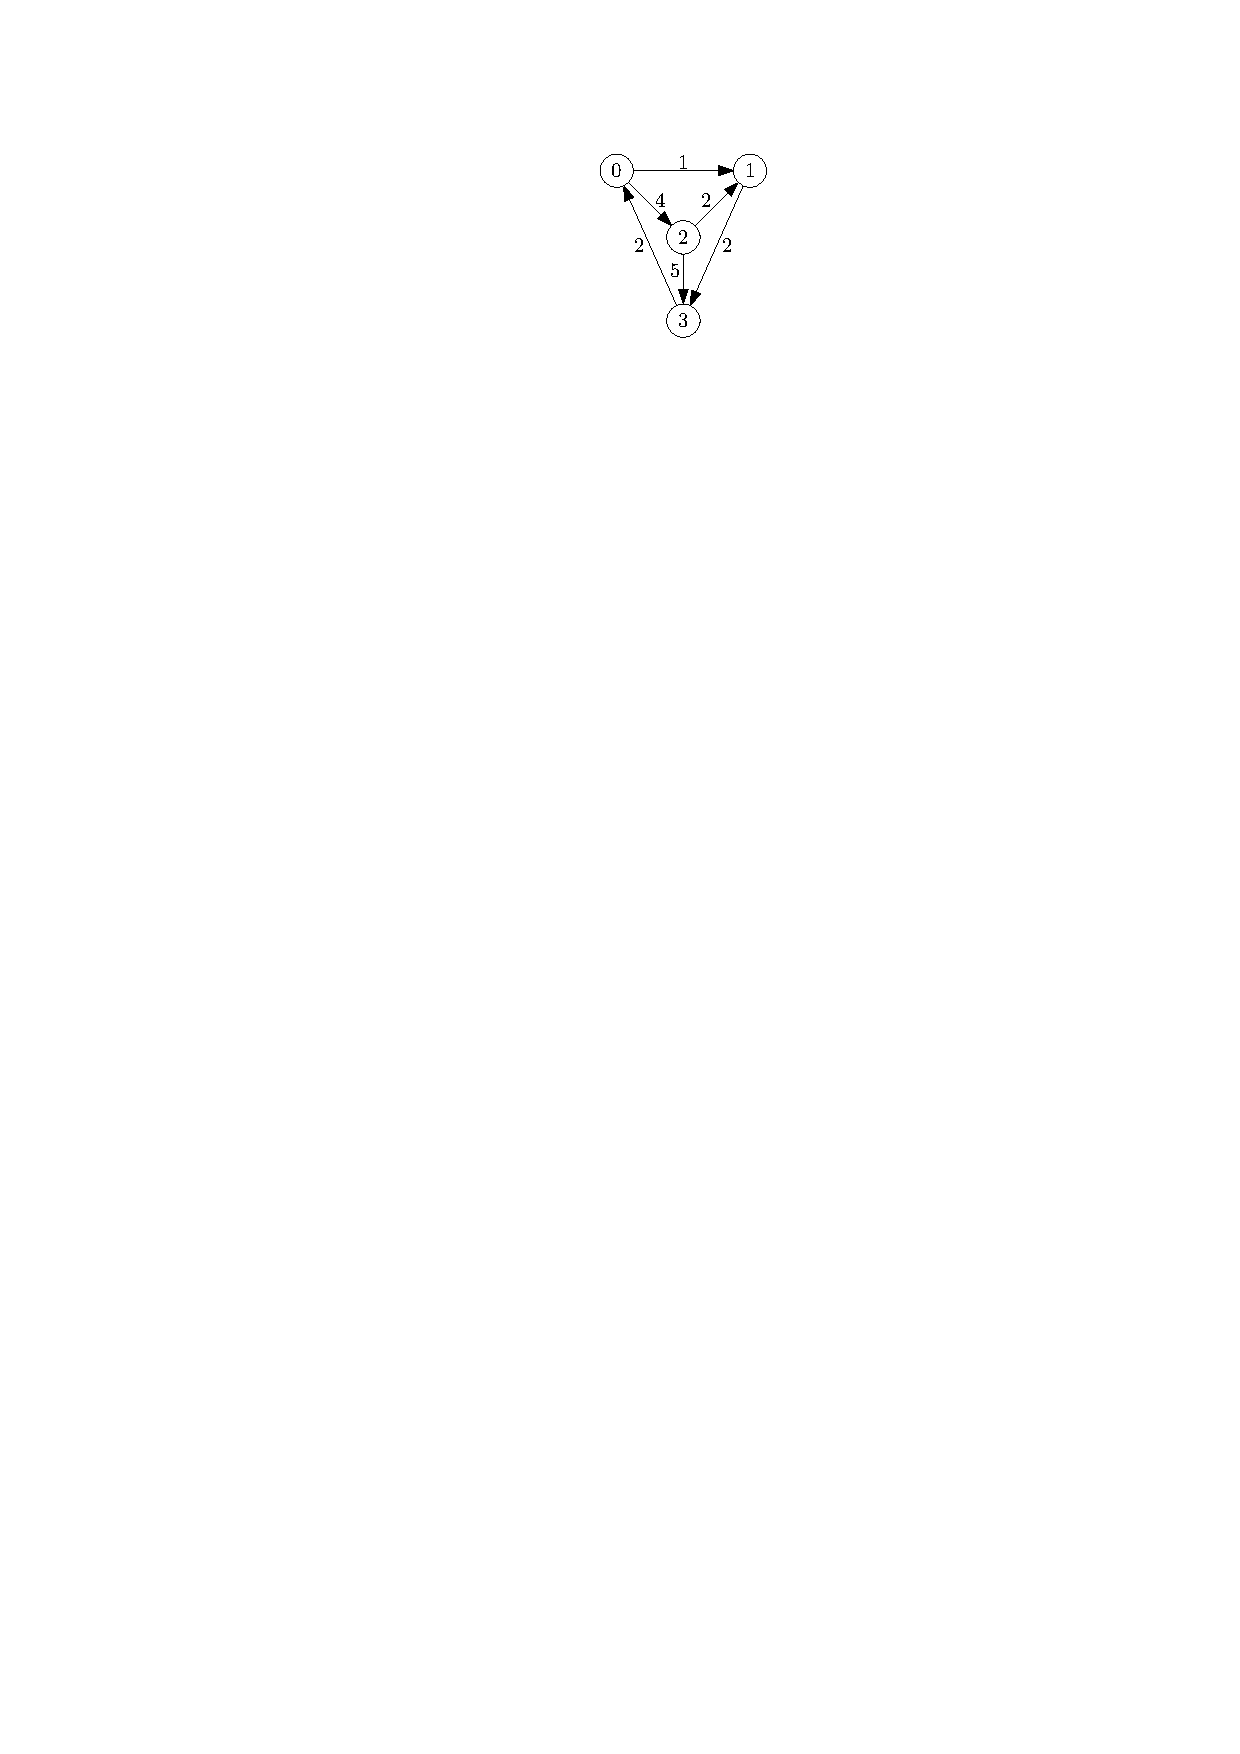
\includegraphics{weightedDigraph}
  \end{center}
  \end{minipage}$\quad$
  \begin{minipage}[c]{0.45\textwidth}
	$$ \left(
	\begin{matrix}
	0 & 1 & 4 & 3 \\
	4 & 0 & 8 & 2 \\
	6 & 2 & 0 & 4 \\
	2 & 3 & 6 & 0
	\end{matrix}
	\right)$$
  \end{minipage}
\end{Boxample}

The APSP problem can be solved by solving the SSSP problem from each node.
\begin{itemize}
  \item If all weights were non-negative, we could run Dijsktra from each of the $n$ nodes, to get a running time of $\Theta(n^3)$.
  \item To be robust to negative weights, using Bellman--Ford gives a $\Theta(n^2 m)$ solution to APSP.
\end{itemize}

\defnfont{Floyd's algorithm} computes a distance matrix from a cost matrix (so solves APSP) in time $\Theta(n^3)$. 
\begin{itemize}
  \item The basic idea is that we find the length of the shortest path between nodes $u$ and $v$ that uses only a fixed set of intermediate nodes. 
  \item This set of intermediate nodes starts at as the empty set (so only arcs from $u$ to $v$ are allowed) and grows, one node at a time, 
until it includes all nodes at which point the algorithm is complete.
  \item It is essentially just a triple for-loop so easy to programme.
  \item Floyd's algorithm is thus faster than Bellman--Ford for non-sparse digraphs.
  \item It is robust to negative weights. 
\end{itemize}

We see how this works in \cref{alg:floydcode} where the outer-for loop iterates through all nodes, essentially adding them to the intermediate set, 
while the inner two loops cycle through all pairs seeing if a shorter path can be found through the new intermediate node.

\begin{algorithm}[H]
  \caption{Floyd's algorithm.}
  \label{alg:floydcode}
\begin{algorithmic}[1]
\Function{Floyd}{weighted digraph $(G, c)$}
	\State array $d[0..n-1,0..n-1]$ \Comment{initialise distance matrix}
	\State $d \gets c$ \Comment{distance matrix starts as copy of weight matrix}
	\For{$x \in V(G)$} \Comment{taking one vertex at a time}
		\For{$u \in V(G)$}
			\For{$v \in V(G)$}
				\State $d[u,v] \gets \min( d[u,v], d[u,x] + d[x,v] )$
				 
				 \Comment{update distance by looking for a shorter path through $x$}
			\EndFor
		\EndFor
	\EndFor
	\State \Return{$d$}
\EndFunction
\end{algorithmic}
\end{algorithm}


\begin{Boxample}[0] \label{eg:floyd}
An application of Floyd's algorithm on the graph on the left is given below.
The initial cost matrix is as follows.

\begin{minipage}[c]{0.45\textwidth}
\centering
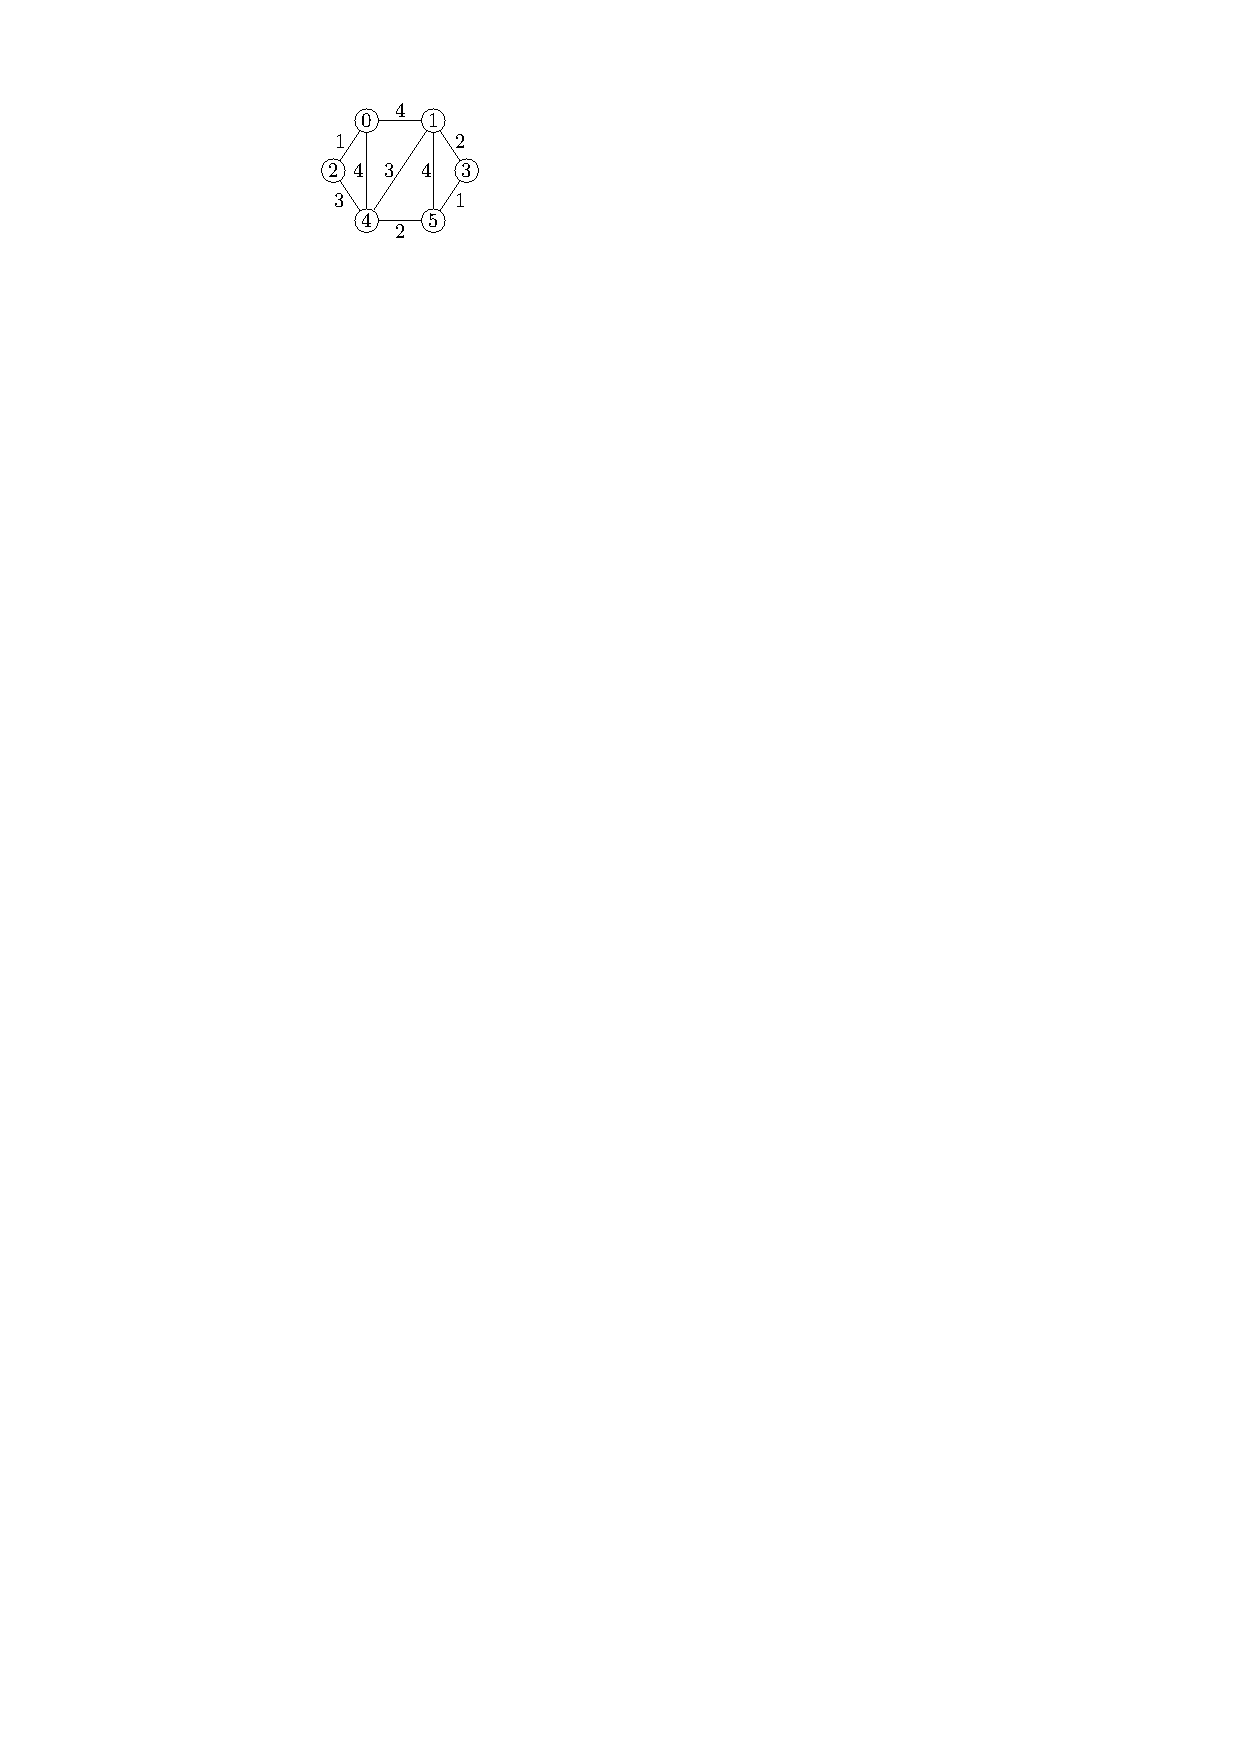
\includegraphics{graphWeighted}
\end{minipage}
\begin{minipage}[c]{0.45\textwidth}
\[ 
\left[
\begin{array}{cccccc} % cost matrix
0        & 4        & 1        & \infty & 4        & \infty \\
4        & 0        & \infty & 2        & 3        & 4 \\
1        &  \infty  & 0        &  \infty  & 3        &  \infty  \\
 \infty  & 2        &  \infty  & 0        &  \infty  & 1 \\
4        & 3        & 3        &  \infty  & 0        & 2 \\
 \infty  & 4        &  \infty  & 1        & 2        & 0 \\
\end{array}
\right]
\hspace{.5cm}
\]
\end{minipage}\\

In the matrices below, we list the entries that change in bold after each iteration of the outer for-loop, 
that is, after $x$ has been $0$, $1$, and so on. 

{\footnotesize
%
\[
\left[
\begin{array}{cccccc} % k = 0
0        & 4        & 1        &  \infty  & 4        &  \infty  \\
4        & 0        & \textbf{5}    & 2        & 3        & 4 \\
1        & \textbf{5}    & 0        &  \infty  & 3        &  \infty  \\
 \infty  & 2        &  \infty  & 0        &  \infty  & 1 \\
4        & 3        & 3        &  \infty  & 0        & 2 \\
 \infty  & 4        &  \infty  & 1        & 2        & 0 \\
\end{array}
\right]
\hspace{.5cm}
\left[
\begin{array}{cccccc} % k = 1
0        & 4        & 1        & \textbf{6}    & 4     & \textbf{8} \\
4        & 0        & 5        & 2        & 3        & 4 \\
1        & 5        & 0        & \textbf{7}    & 3      & \textbf{9} \\
\textbf{6}    & 2        & \textbf{7}    & 0        & \textbf{5}  & 1 \\
4        & 3        & 3        & \textbf{5}    & 0        & 2 \\
\textbf{8}   & 4        & \textbf{9}    & 1        & 2        & 0 \\
\end{array}
\right]
\hspace{.5cm}
\left[
\begin{array}{cccccc} % k = 2
0    & 4   & 1   & 6    & 4    & 8 \\
4    & 0   & 5   & 2    & 3    & 4 \\
1    & 5   & 0   & 7    & 3    & 9 \\
6    & 2   & 7   & 0    & 5    & 1 \\
4    & 3   & 3   & 5    & 0    & 2 \\
8    & 4   & 9   & 1    & 2    & 0 \\
\end{array}
\right]
\]\\[-5pt]
\hspace*{2.25cm}$x = 0$ \hspace{3.45cm} $x = 1$ \hspace{3.1cm} $x = 2$ \\
\[
\left[
\begin{array}{cccccc} % k = 3
0    & 4   & 1   & 6    & 4    & \textbf{7} \\
4    & 0   & 5   & 2    & 3    & \textbf{3} \\
1    & 5   & 0   & 7    & 3    & \textbf{8} \\
6    & 2   & 7   & 0    & 5    & 1 \\
4    & 3   & 3   & 5    & 0    & 2 \\
\textbf{7} &\textbf{3} & \textbf{8} & 1    & 2    & 0 \\
\end{array}
\right]
\hspace{.5cm}
\left[
\begin{array}{cccccc} % k = 4
0    & 4   & 1     & 6    & 4    & \textbf{6} \\
4    & 0   & 5     & 2    & 3    & 3 \\
1    & 5   & 0     & 7    & 3    & \textbf{5} \\
6    & 2   & 7     & 0    & 5    & 1 \\
4    & 3   & 3     & 5    & 0    & 2 \\
\textbf{6} & 3   & \textbf{5} & 1    & 2    & 0 \\
\end{array}
\right]
\hspace{.5cm}
\left[
\begin{array}{cccccc} % k = 5
0    & 4   & 1     & 6    & 4    & 6 \\
4    & 0   & 5     & 2    & 3    & 3 \\
1    & 5   & 0     & \textbf{6} & 3    & 5 \\
6    & 2   & \textbf{6} & 0    & \textbf{3} & 1 \\
4    & 3   & 3     & \textbf{3} & 0    & 2 \\
6    & 3   & 5     & 1    & 2    & 0 \\
\end{array}
\right]
\]\\[-5pt]
\hspace*{2.25cm} $x = 3$ \hspace{3.1cm} $x = 4$ \hspace{3.1cm} $x = 5$
\\
} % footnotesize
\end{Boxample}

\begin{Boxample}[14]
Give the cost matrix for the graph on the left.

\vspace{1.5cm}
$\quad$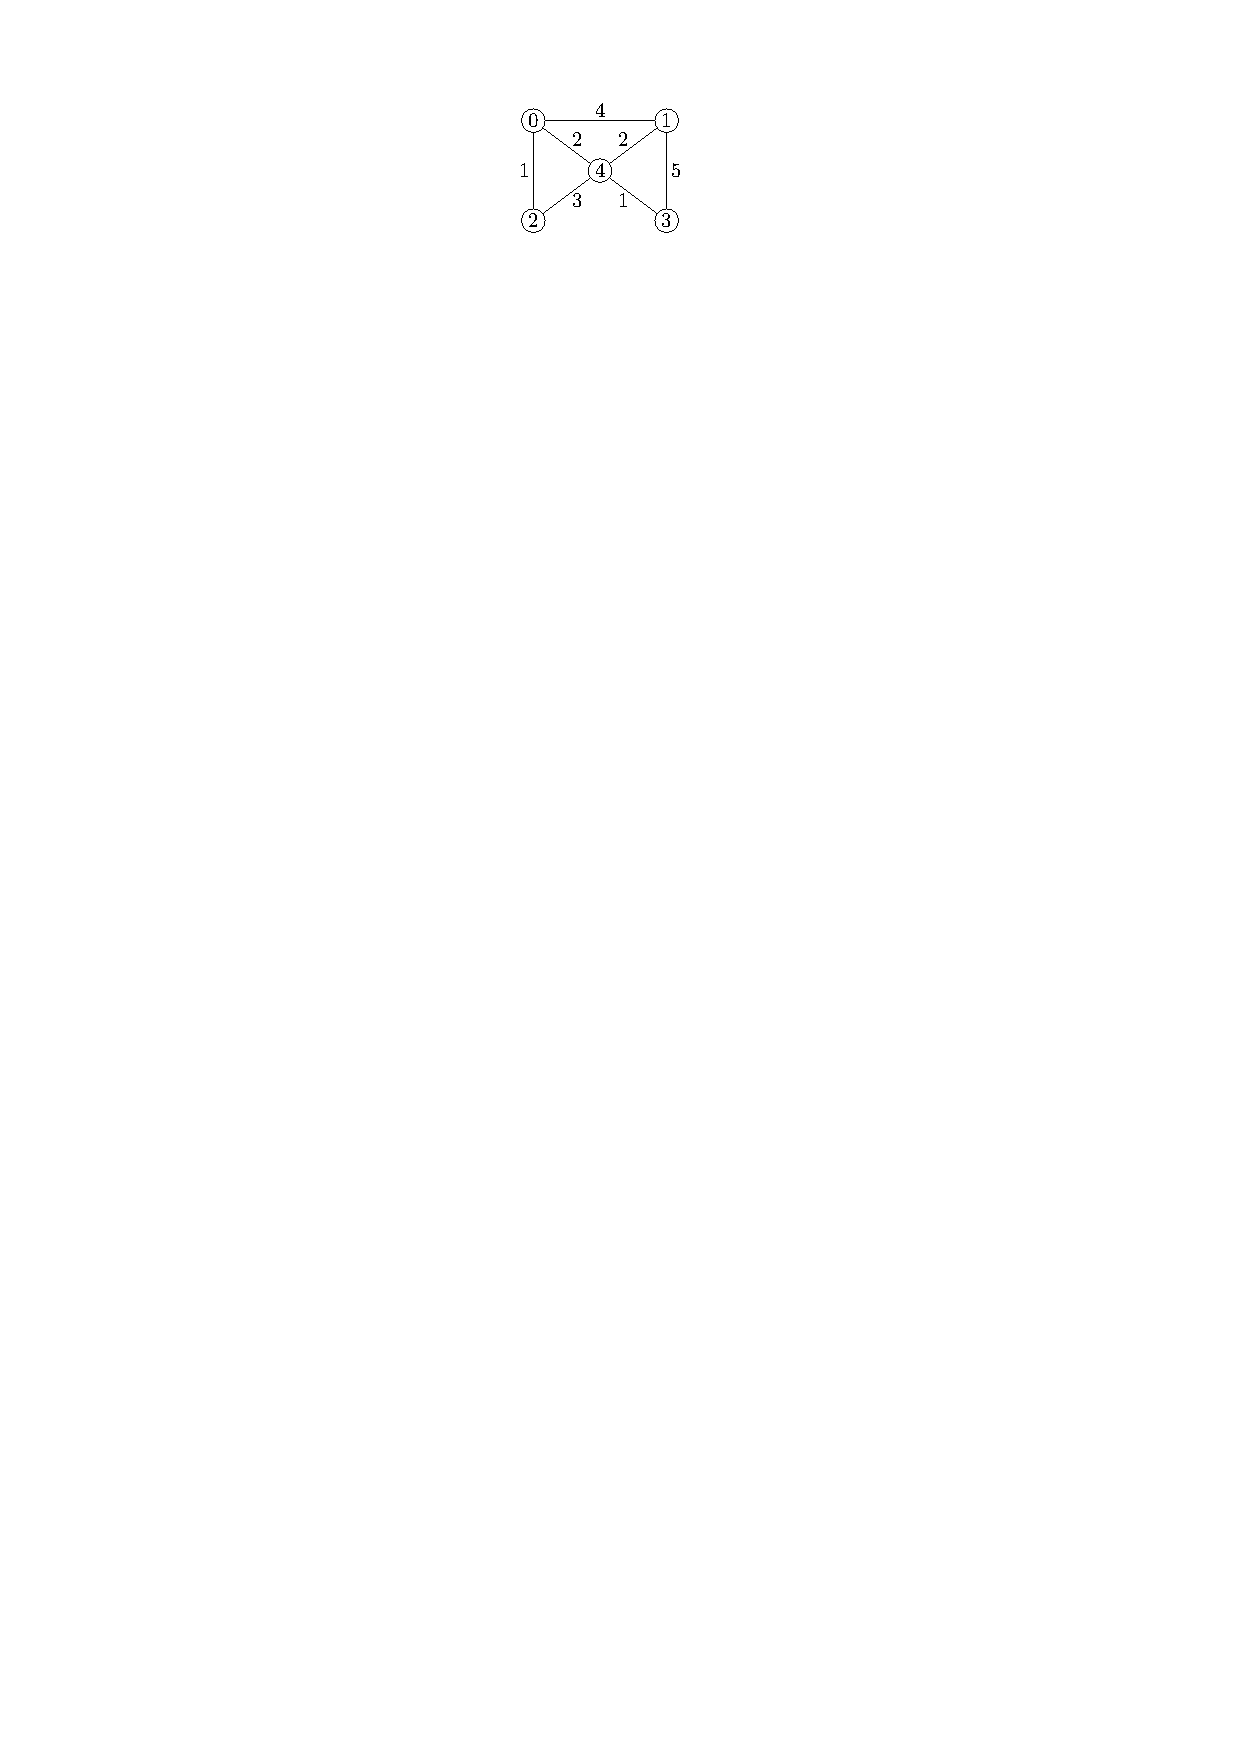
\includegraphics{FloydEx} 

\vspace{1.5cm}
Execute Floyd's algorithm on the graph above by giving the matrices after each iteration of the outer for-loop.

\end{Boxample}

\section{Proof of Floyd's algorithm}
\begin{Theorem} \label{thm:floyd}
At the bottom of the outer \boldfont{for} loop, for all nodes $u$ and $v$,
$d[u,v]$ contains the minimum length of all paths from $u$ to $v$ that
are restricted to using only intermediate nodes that have been seen in
the outer \boldfont{for} loop. 
\end{Theorem}

%\begin{note}
%Given this fact, when the algorithm terminates, all nodes have been seen
%in the outer \boldfont{for} loop and so $d[u,v]$ is the length of a
%shortest path from $u$ to $v$.
%\end{note}
\vspace{-5mm}

\begin{proof}
To establish the above property, we use induction on the outer for-loop.
Let $S_k$ be the set of nodes seen after $k$ times through the
outer loop, and define an $S_k$-path  to be one all of whose
intermediate nodes belong to $S_k$. The corresponding value of $d$ is 
denoted $d_k$. We need to show that for all $k$, after $k$ times through 
the outer for-loop, $d_k[u,v]$ is the minimum length of an $S_k$-path 
from $u$ to $v$. 

When $k=0$, $S_0 = \emptyset$ and the result holds. Suppose
it is true after $k$ times through the outer loop and consider what
happens at the end of the $(k+1)$-st time through the outer loop.
Suppose that $x$ was the last node seen in the outer loop, so $S_{k+1}=
S_k \cup \{x\}$. Fix $u, v\in V(G)$ and let $L$ be the minimum length of
an $S_{k+1}$-path from $u$ to $v$. Obviously $L \leq d_{k+1}[u,v]$; we
show that $d_{k+1}[u,v] \leq L$. 

Choose an $S_{k+1}$-path $\gamma$ from $u$ to $v$ of length $L$. If $x$
is not involved then the result follows by inductive hypothesis. If $x$
is involved, let $\gamma_1, \gamma_2$ be the subpaths from $u$ to $x$
and $x$ to $v$ respectively. Then $\gamma_1$ and $\gamma_2$ are
$S_k$-paths and by the inductive hypothesis, $$L \geq |\gamma_1| +
|\gamma_2| = d_k[u,x] + d_k[x,v] \geq d_{k+1}[u,v]\text{.}$$
\end{proof}

\begin{Boxample}[8]
Draw a table to compare and summarise how BFS, Djikstra, Bellman-Ford and Floyd can be used to solve the SSSP and APSP problems for weighted and unweighted graphs and digraphs with or without negative arcs. Compare their running times and their ability to detect negative cycles.\end{Boxample}

\chapter{Minimum spanning tree problem} %-------------------------------------
\label{sec:MST}
\begin{Definition}
A \defnfont{spanning tree} of a graph $G$ is a subgraph of $G$ that spans $G$ (contains all nodes of $G$) and is a tree (a connected, acyclic graph).

Let $G$ be a weighted graph. 
A \defnfont{minimum spanning tree} (MST) is a spanning tree for $G$ which has minimum total weight 
(sum of all edge weights). 

In the \defnfont{minimum spanning tree problem} we have to find a weighted graph $G$ is to find a MST for $G$. 
\end{Definition}
We can assume throughout that $G$ is connected.

%Note that if all weights are nonnegative and we
%only want a spanning subgraph with minimum total weight, this must be a
%tree anyway. Otherwise we could delete an edge from a cycle and keep a spanning subgraph.

\begin{Boxample}
In the graph below, the tree determined by the edges
$$\{0, 2\}, \{1, 3\}, \{3, 5\}, \{4, 5\}, \{2, 4\}$$ 
has total weight $9$. 
It is a tree and has the $5$ smallest weight edges, so must be a MST.
\begin{center}
  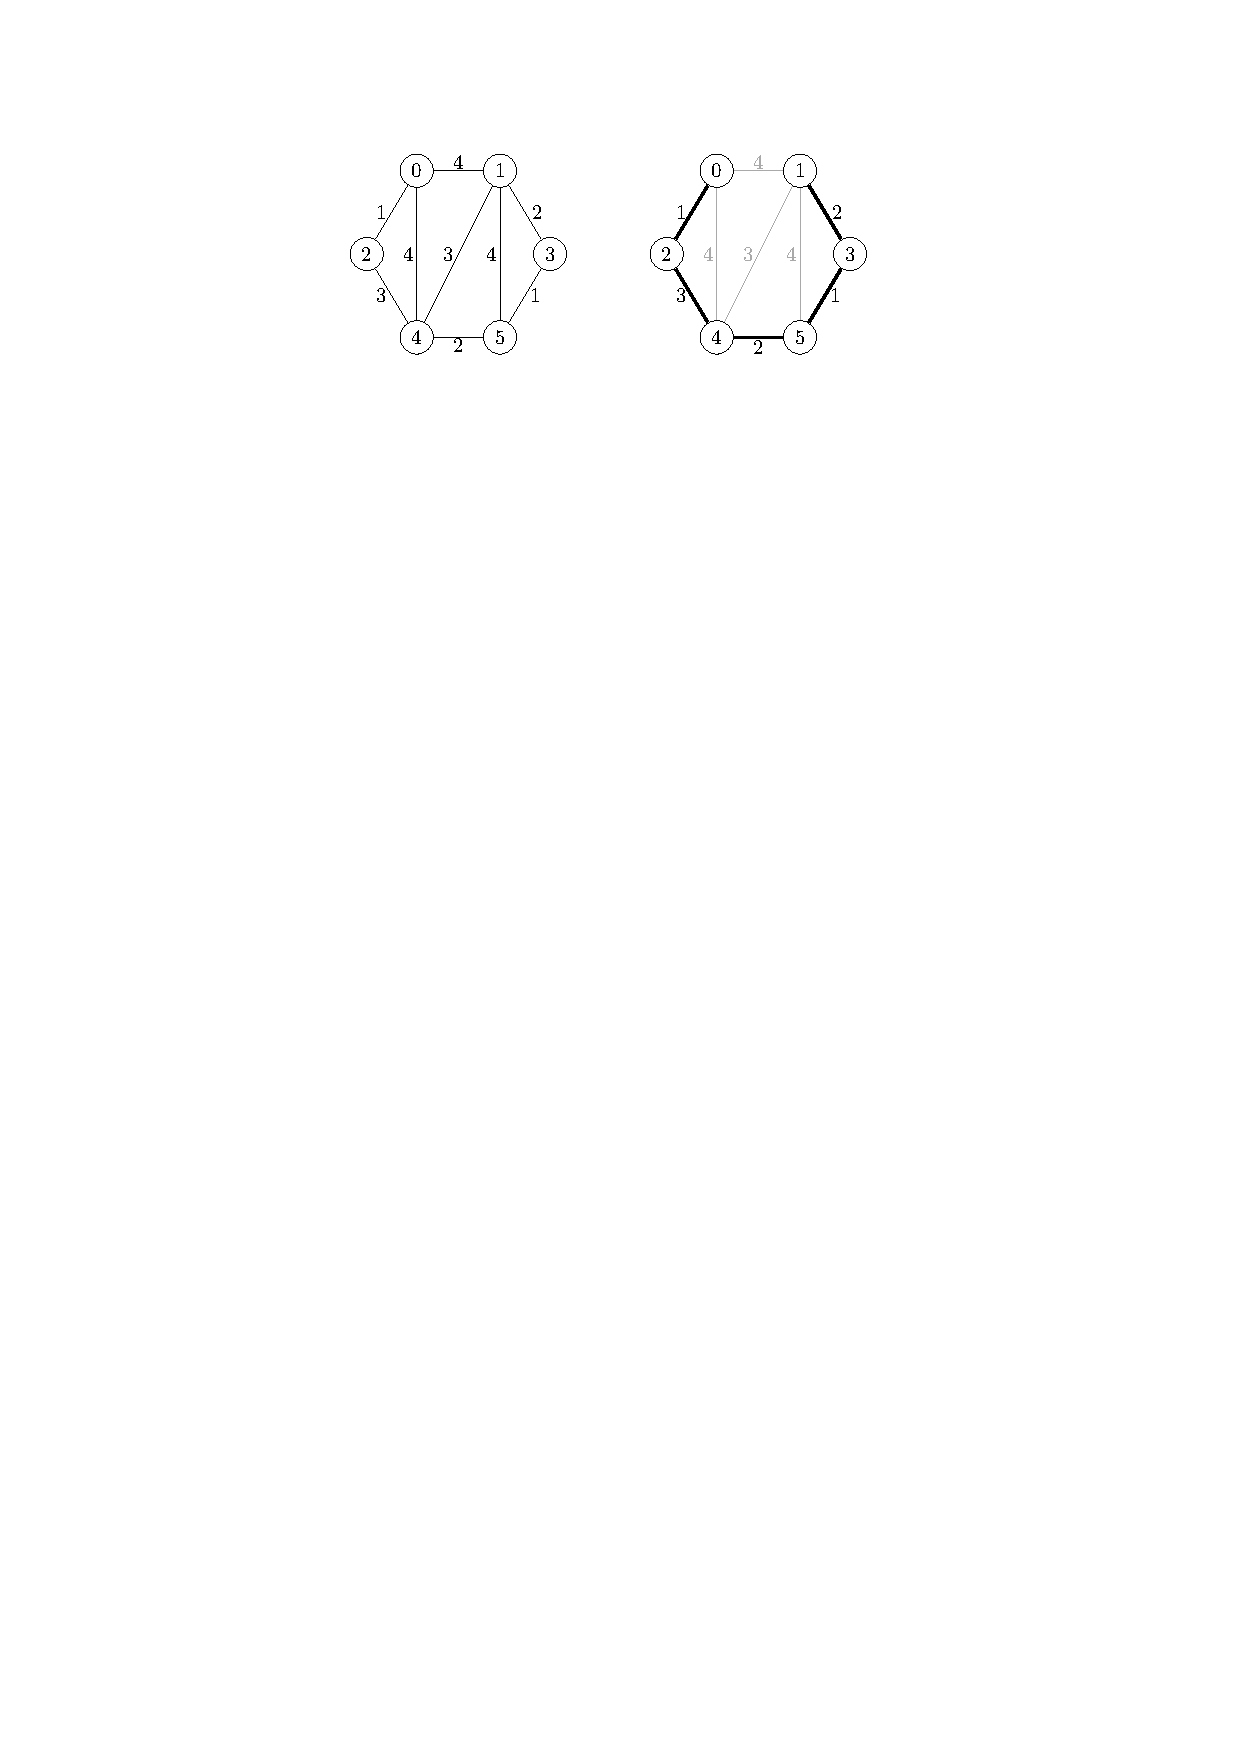
\includegraphics{graphExMST}
\end{center}
\end{Boxample}

We look at two simple greedy algorithms that solve the MST problem.
%Each builds up a MST by iteratively choosing an edge greedily, that is,
%choosing one with minimum weight, subject to not obviously ruining our
%chance of extending to a spanning tree. It turns out that this simple
%approach works for the MST problem (obviously, not for all graph
%optimization problems!). There are other algorithms with better
%theoretical complexity for the MST problem, but none is as simple to
%understand.

\section{Prim's algorithm}
The basic idea of \defnfont{Prim's algorithm} is simple:
\begin{itemize}
\item Start at any vertex.
\item Choose at each step an edge of minimum weight from the remaining edges ensuring that
\begin{enumerate}
\item adding the edge does not create a cycle in the subgraph built so
far; and 
\item the subgraph built so far is connected.
\end{enumerate}
\item Stop when the tree is a spanning tree.
\end{itemize}

Since the subgraph built is acyclic and connected at each stage, it is a tree.
It is also clear that the algorithm halts and as the tree grows by a node at each stage, 
it will eventually include all nodes of $G$, that is, be a spanning tree. 
So the only thing that needs to be proved for correctness is that the tree has the lowest possible weight (is minimum). 
We will prove this but first look at the code.

Pseudocode is given in \cref{alg:primcode}. 
Note how similar Prim's algorithm is to Dijkstra's algorithm. 
The main difference is in the update formula. We also store the PFS tree, which we did not do for Dijkstra.

\begin{algorithm}[H]
  \caption{Prim's algorithm.}
  \label{alg:primcode}
\begin{algorithmic}[1]
\Function{Prim}{weighted graph $(G, c)$; vertex $s\in V(G)$}
	\State priority queue $Q$
	\State array $\colour[0..n-1]$, $\pred[0..n-1]$
	\For{$u \in V(G)$}
		\State $\colour[u] \gets$ WHITE; $\pred[u] \gets$ \texttt{null} 
	\EndFor
	\State $\colour[s] \gets $ GREY
	\State $Q$.\texttt{insert}$(s, 0)$
	\While{\textbf{not} $Q$.\texttt{isEmpty}$()$}
		\State $u \gets Q$.\texttt{peek}$()$
		\For{each $x$ adjacent to $u$}
			\State $t \gets c(u, x)$
			\If{$\colour[x] = $ WHITE}
				\State $\colour[x] \gets $ GREY; $\pred[x] \gets u$
				\State $Q$.\texttt{insert}$(x, t)$
			\ElsIf{$\colour[x] = $ GREY \textbf{and} $Q$.\texttt{getKey}$(x) > t$}
				\State $Q$.\texttt{decreaseKey}$(x, t)$; $\pred[x] \gets u$
			\EndIf
		\EndFor
		\State $Q$.\texttt{delete}$()$
		\State $\colour[u] \gets $ BLACK
	\EndWhile
	\State \Return{$\pred$}
\EndFunction
\end{algorithmic}
\end{algorithm}


\begin{Boxample}
Application of Prim's algorithm on a graph, choosing node with lowest index where there is a choice.
\begin{center}
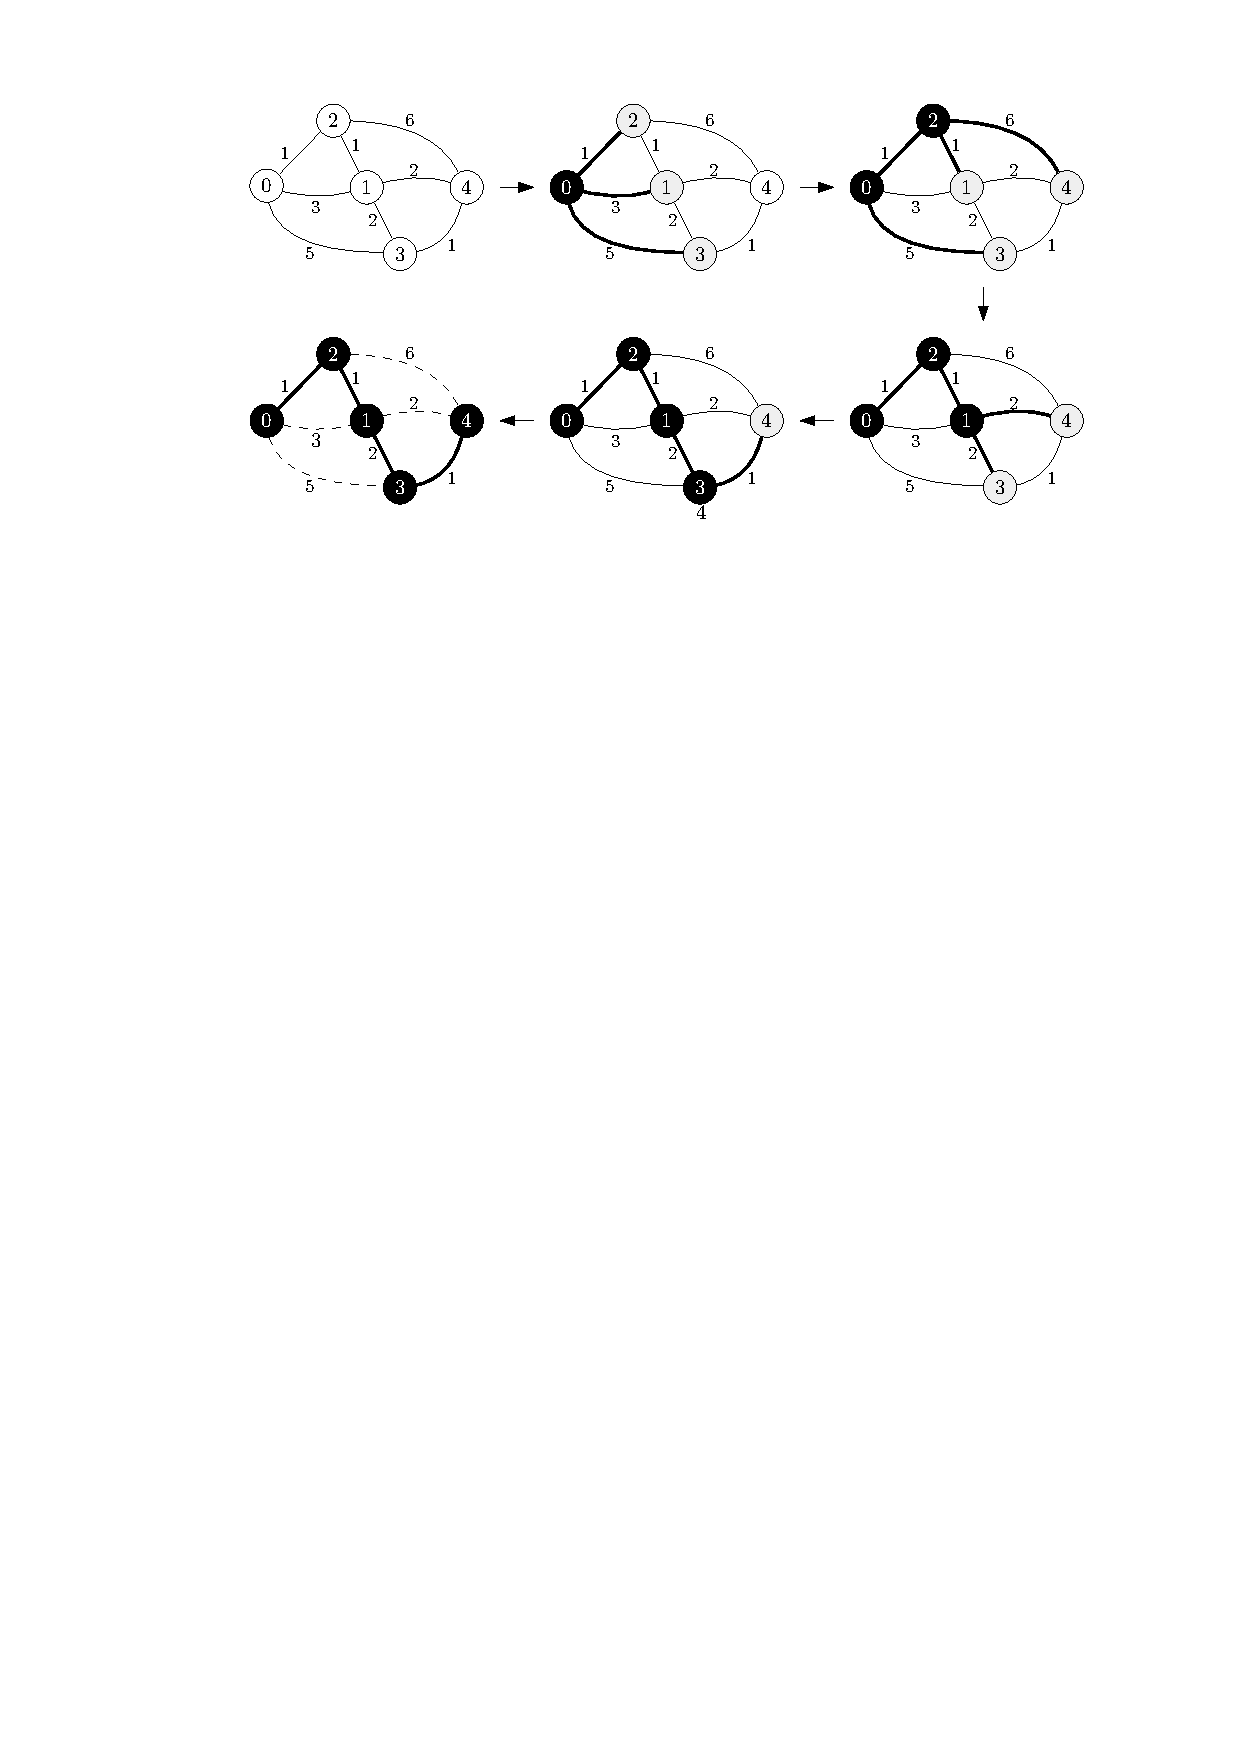
\includegraphics[width=1.0\textwidth]{PrimExUndirected}
\end{center}
\end{Boxample}

\begin{Boxample}[0.2]
Execute Prim's algorithm.\\

\begin{center}
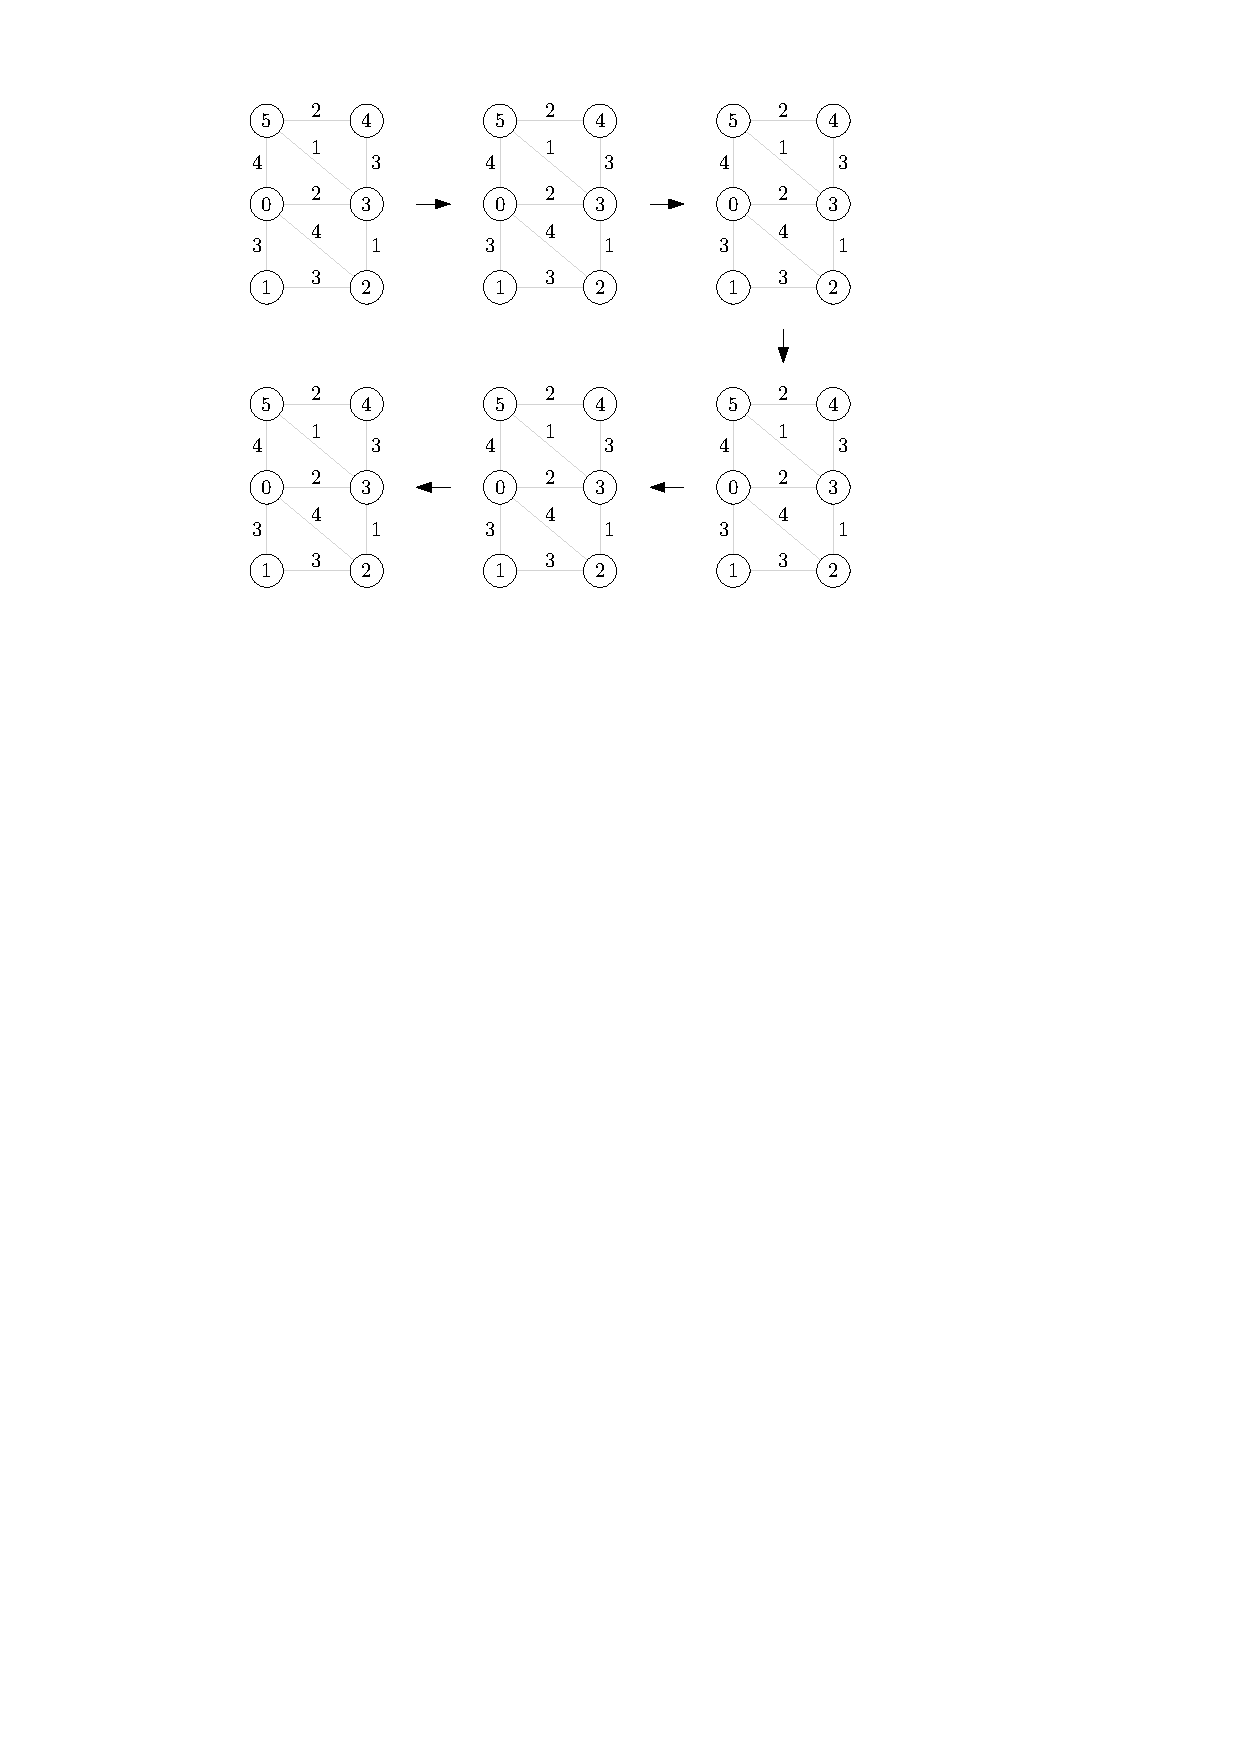
\includegraphics[width=1.0\textwidth]{PrimEx}
\end{center}
\end{Boxample}

%\begin{Theorem} \label{thm:prim}
%Prim's algorithms is correct.
%\end{Theorem}
\begin{Boxample}[17.5]
Prove that Prim's algorithm is correct.
%Define a set of edges to be \boldfont{promising} if it can be extended in some way to a MST. 
%Then the empty set is promising since some MST exists. 
%We claim that at each step, the algorithms above have chosen a promising set of edges. 
%When they terminate, no further extension of the set is possible (by rule (a) above), 
%and so we must have a MST.
%
%To prove the claim efficiently, we need a technical fact, as follows.
%Suppose that $B$ is a subset of $V(G)$, not containing all the vertices
%of $G$, and $T$ a promising set of edges such that no edge in $T$ leaves
%$B$. In other words, either both endpoints are in $B$ or neither
%endpoint is in $B$. Then if $e$ is a minimum weight edge that does leave
%$B$ (it has one endpoint in $B$ and one outside) then $T\cup\{e\}$ is
%also promising.
%
%To see this fact, note that since $T$ is promising, it is contained in
%some MST, $U$ say. If $e\in U$ there is nothing to prove. Otherwise,
%when we add $e$ to $U$ we create exactly one cycle. There must be at
%least one other edge, say $e'$, that leaves $B$, otherwise the cycle
%could not close. If we remove $e'$ we obtain a new tree that spans $G$
%and whose total weight is no greater than the total weight of $U$. Thus
%$V$ is also a MST, and since it contains $T\cup\{e\}$, that set is
%promising.
%
%Now to prove the claim, suppose that our algorithm has maintained a
%promising set $T$ of edges so far, and it has just chosen edge $e=\{u,v\}$.
%If we take $B$ at each step to be the set of vertices in the tree (Prim)
%or the set of vertices in the tree containing $u$ (Kruskal), then we may
%apply the fact above to conclude that $T \cup \{e\}$ is promising. This
%concludes the proof of correctness.
\end{Boxample}

\subsection{Running time}
The complexity of the algorithm depends to a great extent on the data
structure used. The best known for Prim is the same as for Dijkstra
and we  get a running time in $O(m + n\log n)$.

\section{Kruskal's algorithm}

\defnfont{Kruskal's algorithm} is even simpler than Prim's to state.
\vspace{-1.5mm}
\begin{itemize}
\item Start with an empty set of edges.
\item At each step choose an edge of minimum weight from the remaining edges ensuring 
that adding the edge does not create a cycle in the subgraph built so far. 
\item Stop when the subgraph is spanning tree.
\end{itemize}
\vspace{-1.5mm}
Kruskal's algorithm maintains acyclicity, so it has a forest
at each step, and the different trees merge as the algorithm progresses.

\begin{algorithm}[H]
  \caption{Kruskal's algorithm.}
  \label{alg:kruskal}
\begin{algorithmic}[1]
\Function{Kruskal}{weighted digraph $(G, c)$}
	\State disjoint sets ADT $A$
	\State initialize $A$ with each vertex in its own set
	\State sort the edges in increasing order of cost
	\For{each edge $\{u, v\}$ in increasing cost order}
		\If{\textbf{not} $A$.\texttt{set}$(u) = A$.\texttt{set}$(v)$}
			\State add this edge
			\State $A$.\texttt{union}$(A$.\texttt{set}$(u)$, $A$.\texttt{set}$(v))$
		\EndIf
	\EndFor
	\State \Return{$A$}
\EndFunction
\end{algorithmic}
\end{algorithm}

\begin{Boxample}
Application of Kruskal's algorithm on a graph shown until an MST is found. 
Note that the edge \set{0, 2} with weight $2$ is not added, 
because $0$ and $2$ are already in the same set in $A$.\\
\begin{center}
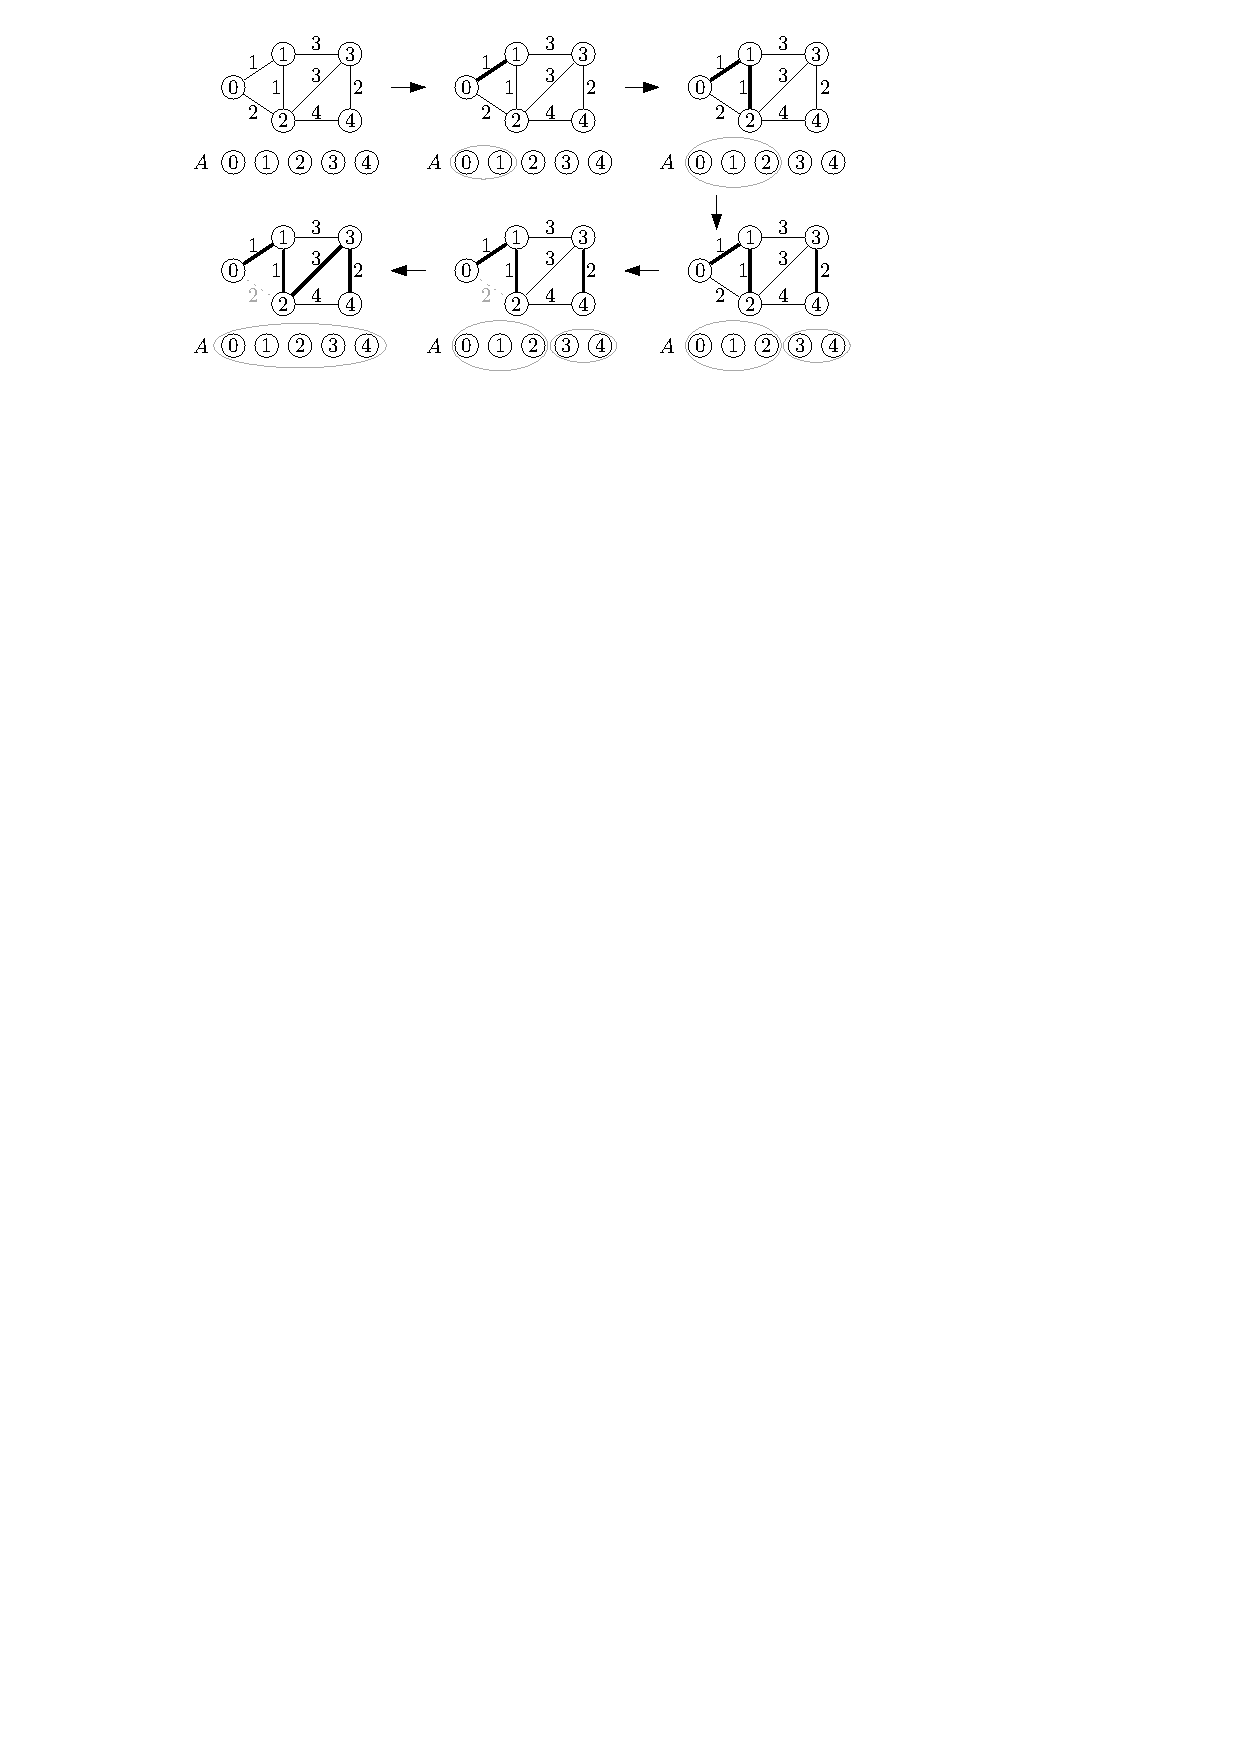
\includegraphics[width=1.0\textwidth]{KruskalEx3}
\end{center}
\end{Boxample}

\begin{Boxample}[0.2]
Execute Kruskal's algorithm by adding or crossing out the next edge. Stop when you reached an MST.\\

\begin{center}
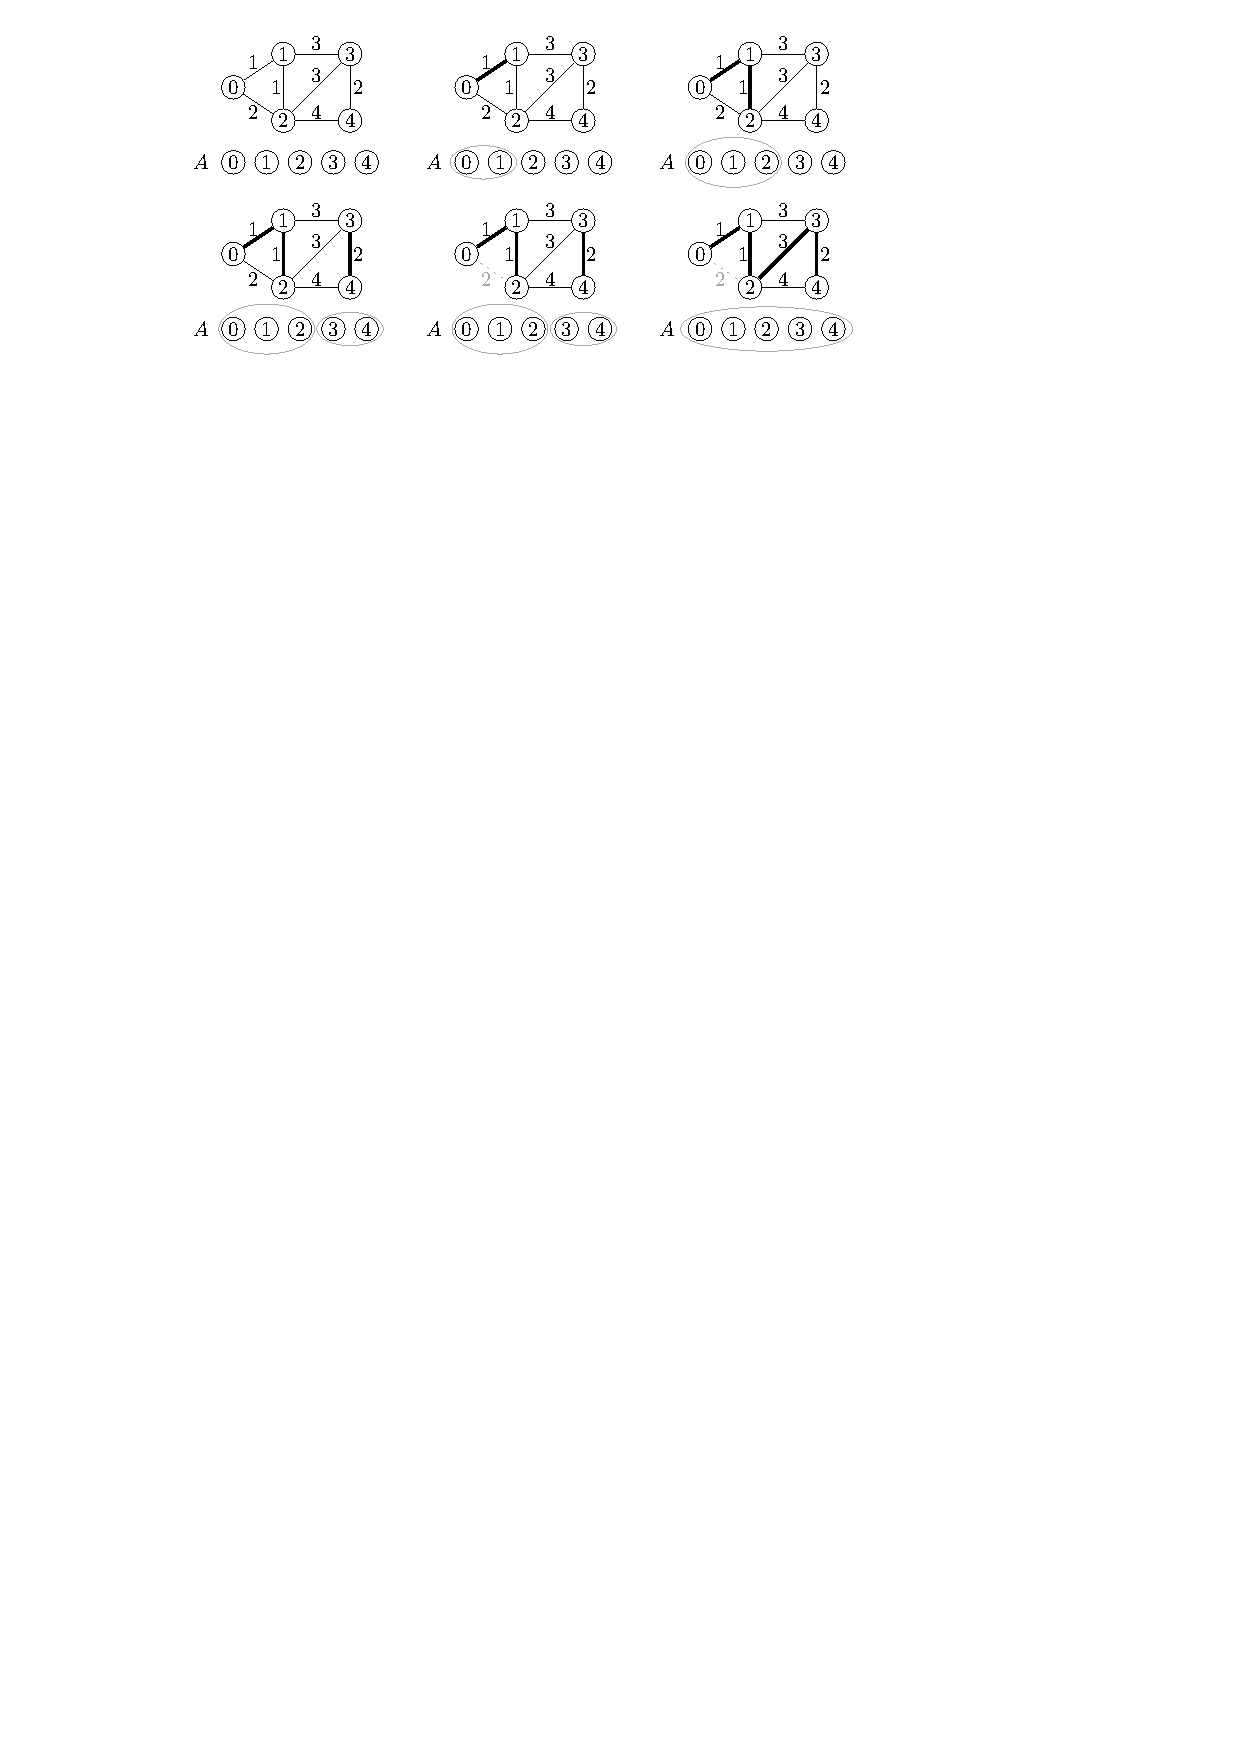
\includegraphics[width=1.0\textwidth]{KruskalEx2}
\end{center}
\end{Boxample}

%In Prim's algorithm, we checked whether a cycle would be created by adding
%an edge in the usual way: when exploring $\{u, v\}$ from $u$, if $v$ has
%already been seen and is not the parent of $u$, then adding $\{u, v\}$
%creates a cycle. With Kruskal's algorithm, we must use another method,
%since the above test does not work. Both $u$ and $v$ may have been seen,
%but may be in different trees.

Observe that if we try to add an edge both of whose endpoints are in
the same tree in the Kruskal forest, this will create a cycle, so the
edge must be rejected. On the other hand, if the endpoints are in two
different trees, a cycle definitely will not be created; rather, the two
trees merge into a single one, and we should accept the edge. 

We need a data structure that can handle this efficiently. All we need is to be
able to find the tree containing an endpoint, and to merge two trees. The
\defnfont{disjoint sets} or \defnfont{union-find} ADT is precisely what
is needed. It allows us to perform the \texttt{find} and \texttt{union}
operations efficiently. We do not look at the details of this ADT here.



Kruskal's is in $O(m \log n)$ using the disjoint sets ADT. 
The ADT can be implemented in such a way that the union and find operations
in Kruskal's algorithm runs in \boldfont{almost} linear time. So if the edge weights are presorted, or can be
sorted in linear time (for example, if they are known to be integers in
a fixed range), then Kruskal's algorithm runs for practical purposes in
linear time.



\chapter{Hard graph problems}%------------------------------------------------
\label{sec:hardgraph}
All of the problems we have considered so far have solutions whose running time is  bounded above by a low
degree polynomial in the size of the input. However, there are many
essential problems that currently do not have known polynomial-time
algorithms (so-called \defnfont{NP-hard} problems). Some examples
are:
\begin{itemize}
\item finding the longest path between two nodes of a digraph;
\item finding a $k$-colouring of a graph, for fixed $k \geq 3$;
\item finding a cycle that passes through all the vertices of
a graph (a \defnfont{Hamiltonian cycle});
\item finding a
minimum weight path that passes through all the vertices of a weighted
digraph (the \defnfont{travelling salesperson problem} or TSP);
\item finding the largest \defnfont{independent set} in a graph, that is, 
a subset of vertices no two of which are connected by an edge;
\item finding the smallest \defnfont{vertex cover} of a graph, that is, a special subset of
vertices so that each vertex of the graph is adjacent to one in that
subset. 
\end{itemize}

Investigating these problems is an active research area in computer
science. In many cases the only approach known to the general problem is to try
all possibilities, with some rules that prevent the listing of obviously
hopeless ones. In some special cases (for example, if a graph is bipartite, the vertex cover problem is solvable in polynomial time)
or where the graph is in some sense ``close to" a tree, much faster algorithms can be developed.

